%%%%%%%%Bilecik Şeyh Edebali Üniversitesi Mühendsilik Fakültesi%%%% 
%%%%%%%%Bilgisayar Mühendisliği Bitirme Çalışması%%%%%%%%%%%%%%%%%%
%%%%%%%%%%%%%%%%%%%%%%LaTeX Class%%%%%%%%%%%%%%%%%%%%%%%%%%%%%%%%%%
\documentclass{BUB}

\usepackage{subcaption}
\usepackage{longtable}

% JSON için listings tanımı
\lstdefinelanguage{json}{
    basicstyle=\normalfont\ttfamily,
    numbers=left,
    numberstyle=\scriptsize,
    stepnumber=1,
    numbersep=8pt,
    showstringspaces=false,
    breaklines=true,
    frame=lines,
    backgroundcolor=\color{gray!10},
    literate=
     *{0}{{{\color{blue}0}}}{1}
      {1}{{{\color{blue}1}}}{1}
      {2}{{{\color{blue}2}}}{1}
      {3}{{{\color{blue}3}}}{1}
      {4}{{{\color{blue}4}}}{1}
      {5}{{{\color{blue}5}}}{1}
      {6}{{{\color{blue}6}}}{1}
      {7}{{{\color{blue}7}}}{1}
      {8}{{{\color{blue}8}}}{1}
      {9}{{{\color{blue}9}}}{1}
      {:}{{{\color{red}:}}}{1}
      {,}{{{\color{red},}}}{1}
      {\{}{{{\color{red}\{}}}{1}
      {\}}{{{\color{red}\}}}}{1}
      {[}{{{\color{red}[}}}{1}
      {]}{{{\color{red}]}}}{1},
    string=[s]{"}{"},
    stringstyle=\color{green},
    comment=[l]{//},
    commentstyle=\color{gray},
}

% YAML için listings tanımı
\lstdefinelanguage{yaml}{
    keywords={true,false,null,y,n},
    keywordstyle=\color{darkgray}\bfseries,
    basicstyle=\YAMLkeystyle,
    sensitive=false,
    comment=[l]{\#},
    morecomment=[s]{/*}{*/},
    commentstyle=\color{purple}\ttfamily,
    stringstyle=\YAMLvaluestyle\ttfamily,
    moredelim=[l][\color{orange}]{\&},
    moredelim=[l][\color{magenta}]{*},
    moredelim=**[il][\YAMLcolonstyle{:}\YAMLvaluestyle]{:},
    morestring=[b]',
    morestring=[b]",
    literate =    {---}{{\ProcessThreeDashes}}3
                  {>}{{\textcolor{red}{\textgreater}}}1     
                  {|}{{\textcolor{red}{\textbar}}}1 
                  {\ -\ }{{\mdseries\ -\ }}3,
}

% Groovy için listings tanımı
\lstdefinelanguage{groovy}{
    keywords={abstract,break,case,catch,class,const,continue,def,default,do,else,extends,false,finally,for,goto,if,implements,import,instanceof,interface,native,new,null,package,private,protected,public,return,static,super,switch,synchronized,this,throw,throws,transient,true,try,void,volatile,while},
    keywordstyle=\color{blue}\bfseries,
    ndkeywords={boolean,byte,char,double,float,int,long,short,void,String},
    ndkeywordstyle=\color{darkgray}\bfseries,
    identifierstyle=\color{black},
    sensitive=false,
    comment=[l]{//},
    morecomment=[s]{/*}{*/},
    commentstyle=\color{purple}\ttfamily,
    stringstyle=\color{red}\ttfamily,
    morestring=[b]',
    morestring=[b]"
}

% YAML stil komutları
\newcommand\YAMLcolonstyle{\color{red}\mdseries}
\newcommand\YAMLkeystyle{\color{black}\bfseries}
\newcommand\YAMLvaluestyle{\color{blue}\mdseries}
\makeatletter
\newcommand\ProcessThreeDashes{\llap{\color{cyan}\mdseries-{-}-}}
\makeatother

%%%%%%%%%%%%%%%%%%%%%%%%%%%%%%%%%%%%%%%%%%%%%%%%%%%%%%%%%%%%%%%%%%%
\begin{document}
%%%%%%%%%%%%%%%%%%%%%%Bitirme Çalışmasının Bölümleri%%%%%%%%%%%%%%% 
% \include{1diskapak}
\thispagestyle{empty}
    \begin{center}

    \textbf{T.C. \\BİLECİK ŞEYH EDEBALİ ÜNİVERSİTESİ \\ MÜHENDİSLİK FAKÜLTESİ \\ BİLGİSAYAR MÜHENDİSLİĞİ BÖLÜMÜ}
    \vspace{.75cm}
    
    \begin{figure}[h!]
    \centering
    
\includegraphics[width=0.25\linewidth]{BSEU_LOGO.png}   
    \end{figure}
    
    \vspace{1.25cm}
    
    \textbf{CORAZA WAF LOG ANALİZİ VE SOM KÜMELEMESİ İLE GÜVENLİK TEHDİT TESPİTİ SİSTEMİ }

    \vspace{2cm}
    
    \textbf{Zübeyir TOSUN} \\
    
    \vfill
    \textbf{DANIŞMAN} \\    
    \textbf{Öğr. Gör. Zafer SERİN} \\
    
    \vspace{0.8cm}
    % \textbf{BM400 Bitirme Çalışması}
    % \textbf{BM331 Bilgisayar Mühendisliği Tasarım Çalışması I}
    \textbf{BM328 Bilgisayar Mühendisliği Tasarım Çalışması II}
    \vspace{0.8cm}
    
    
    \textbf{BİLECİK \the\year}
    \end{center}

\pagenumbering{roman} % romen rakamları kullanılmaya başlanıyor.
\setcounter{page}{2}  % sayfa numarasını ii'den başlatılıyor.
\begin{center}
\textbf{BİLDİRİM}
\end{center}
\begin{singlespace}%1 satır aralığı
Bu çalışmada bütün bilgilerin etik davranış ve akademik kurallar çerçevesinde elde edildiğini ve yazım kurallarına uygun olarak hazırlanan bu çalışmada bana ait olmayan her türlü ifade ve bilginin kaynağına eksiksiz atıf yapıldığını bildiririm.
\end{singlespace}
\vspace{2cm}

\begin{center}
\textbf{DECLARATION}
\end{center}
\begin{singlespace}
I hereby declare that all information in this document has been obtained and presented in accordance with academic rules and ethical conduct. I also declare that, as required by these rules and conduct, I have fully cited and referenced all materials and results that are not original to this work.
\end{singlespace}

\vspace{3cm}
\begin{flushright}
\begin{minipage}{5cm}
\begin{center}
\textbf{İmza}

\textbf{Zübeyir TOSUN}

\textbf{Tarih: {18 Haziran 2025}}\hfill
\end{center}
\end{minipage}
\end{flushright}


%-----------------------------------------------------%
\pagenumbering{roman}
\newpage
\begin{center}
\large \textbf{ÖZET}
\end{center}

Bu çalışmada, Coraza WAF log kayıtlarını SOM algoritması ile analiz ederek anormal davranış kalıplarını tespit eden ve güvenlik olaylarını görselleştiren bir sistem geliştirilmiştir. Sistem, Jenkins entegrasyonu ile sürekli entegrasyon/sürekli dağıtım (CI/CD) pipeline'ı üzerinde çalışmakta ve OWASP ZAP (Zed Attack Proxy) ile otomatik güvenlik taramalarını gerçekleştirmektedir.

Geliştirilen sistemin temelinde Self-Organizing Map (SOM) algoritması kullanılarak log verilerinin kümelenmesi ve anormal davranışların tespiti yer almaktadır. SOM, yüksek boyutlu log verilerini iki boyutlu bir haritada görselleştirerek benzer davranış kalıplarını gruplandırmakta ve potansiyel güvenlik tehditlerini vurgulamaktadır. Sistem, adaptif grid boyutlandırma formülü ($\sqrt{5 \cdot \sqrt{n}}$) ile otomatik parametre optimizasyonu sağlamaktadır.

Sistem, Streamlit framework'ü üzerinde geliştirilmiş interaktif web arayüzü ile kullanıcılara kapsamlı log analizi, görselleştirme ve raporlama imkanları sunmaktadır. Jenkins otomasyonu sayesinde Coraza WAF ve OWASP Core Rule Set (CRS) kurulumları otomatik olarak gerçekleştirilmekte, güvenlik taramaları periyodik olarak yapılmakta ve sonuçlar JSON formatında log dosyalarına kaydedilmektedir.

Geliştirilen sistem, 2,000 kayıtlık gerçek ZAP Scanner güvenlik test verisi ile doğrulanmış olup, DBSCAN algoritması 0.985 silhouette skor ile yüksek performans sergilemiştir. Meta-kümeleme (K-means, DBSCAN, Hierarchical), boyut indirgeme (PCA, t-SNE, UMAP), anomali tespiti ve PDF rapor üretimi gibi gelişmiş analiz modülleri entegre edilmiştir. Sistem, farklı JSON formatlarını işleyebilmekte ve gerçek güvenlik verisi üzerinde etkili analiz sonuçları üretmektedir.

\textbf{Anahtar Kelimeler:} Web Application Firewall, Self-Organizing Map, Log Analizi, Jenkins CI/CD, OWASP ZAP, Güvenlik Analizi, Anomali Tespiti, Meta-Kümeleme, Boyut İndirgeme

\newpage
\begin{center}
\large \textbf{ABSTRACT}
\end{center}

In this study, a system has been developed that analyzes Coraza WAF log records using the SOM algorithm to detect abnormal behavior patterns and visualize security events. The system operates on a continuous integration/continuous deployment (CI/CD) pipeline with Jenkins integration and performs automated security scans using OWASP ZAP (Zed Attack Proxy).

The core of the developed system is based on clustering log data and detecting anomalous behaviors using the Self-Organizing Map (SOM) algorithm. SOM visualizes high-dimensional log data on a two-dimensional map, grouping similar behavior patterns and highlighting potential security threats. The system provides automatic parameter optimization with adaptive grid sizing formula ($\sqrt{5 \cdot \sqrt{n}}$).

The system provides users with comprehensive log analysis, visualization, and reporting capabilities through an interactive web interface developed using the Streamlit framework. Through Jenkins automation, Coraza WAF and OWASP Core Rule Set (CRS) installations are performed automatically, security scans are conducted periodically, and results are recorded in log files in JSON format.

The developed system has been validated with 2,000 real ZAP Scanner security test data records, with the DBSCAN algorithm achieving high performance with a 0.985 silhouette score. Advanced analysis modules such as meta-clustering (K-means, DBSCAN, Hierarchical), dimensionality reduction (PCA, t-SNE, UMAP), anomaly detection, and PDF report generation have been integrated. The system can process different JSON formats and produces effective analysis results on real security data.

\textbf{Keywords:} Web Application Firewall, Self-Organizing Map, Log Analysis, Jenkins CI/CD, OWASP ZAP, Security Analysis, Anomaly Detection, Meta-Clustering, Dimensionality Reduction

\pagebreak{}



\phantomsection
\section*{ÖNSÖZ}
\addcontentsline{toc}{section}{ÖNSÖZ}
\vspace{.5cm}
Bitirme çalışmamın başından sonuna kadar emeği geçen ve beni bu konuya yönlendiren saygı değer hocam ve danışmanım Sayın Ünvan Ögr. Gör. Zafer SERİN’e tüm katkılarından ve hiç eksiltmediği desteğinden dolayı teşekkür ederim.

\vspace{2cm}
\begin{flushright}
\begin{minipage}{5cm}
\begin{center}
\textbf{İmza}

\textbf{Zübeyir TOSUN}

\textbf{Tarih: {\today}}\hfill
\end{center}
\end{minipage}
\end{flushright}

%%%İçindekiler ve tablolar%%%%%%%%%%%%%%
\phantomsection
\addcontentsline{toc}{section}{İÇİNDEKİLER}
\tableofcontents
%%%%%%%%%%%%%%%%ŞEKİLLER DİZİNİ%%%%%%%%%%%%%%
\phantomsection
\renewcommand*\listfigurename{\centerline{\normalsize ŞEKİLLER DİZİNİ}}
\addcontentsline{toc}{section}{\normalsize ŞEKİLLER DİZİNİ}
\listoffigures%bu komutun olduğu yerde şekiller listesi oluşturulur
%%%%%%%%%%%%%%%%%%%%%TABLOLAR DİZİNİ%%%%%%%%%%%%%%%%%
\phantomsection
\renewcommand*\listtablename{\centerline{\normalsize TABLOLAR DİZİNİ}}
\listoftables%bu komutun olduğu yerde tablolar listesi oluşturulur
\addcontentsline{toc}{section}{TABLOLAR DİZİNİ}
%%%%%%%%%%%%%%%%%%%%%TABLOLAR DİZİNİ%%%%%%%%%%%%%%%%%
\phantomsection
\section*{SİMGELER VE KISALTMALAR}
\addcontentsline{toc}{section}{SİMGELER VE KISALTMALAR}

\begin{spacing}{1.0}
\begin{longtable}{@{}p{0.25\textwidth} p{0.7\textwidth}@{}}
\textbf{BMU}  &	En İyi Eşleşen Birim (Best Matching Unit) \\[1ex]
\textbf{Bootstrap} & İstatistiksel yeniden örnekleme yöntemi \\[1ex]
\textbf{CH} & Calinski-Harabasz İndeksi \\[1ex]
\textbf{CI/CD}  &	Sürekli Entegrasyon/Sürekli Dağıtım \\[1ex]
\textbf{Coraza} & Modern Web Uygulaması Güvenlik Duvarı Motoru \\[1ex]
\textbf{CRS}  &	Temel Kural Seti (Core Rule Set) \\[1ex]
\textbf{DB} & Davies-Bouldin İndeksi \\[1ex]
\textbf{DBSCAN}  &	Gürültülü Uygulamaların Yoğunluk Tabanlı Uzamsal Kümelenmesi \\[1ex]
\textbf{Dendrogram} & Hiyerarşik kümeleme ağaç diyagramı \\[1ex]
\textbf{Docker} & Konteynerleştirme platformu \\[1ex]
\textbf{Flask} & Python mikro web çerçevesi \\[1ex]
\textbf{FPDF}  &	Özgür PDF Üretici Kütüphanesi \\[1ex]
\textbf{Go} & Google tarafından geliştirilen programlama dili \\[1ex]
\textbf{Groovy} & Jenkins boru hattı betik dili \\[1ex]
\textbf{HTML}  &	Köprü Metni İşaretleme Dili \\[1ex]
\textbf{HTTP}  &	Köprü Metni Aktarım Protokolü \\[1ex]
\textbf{Jenkins} & CI/CD otomasyon platformu \\[1ex]
\textbf{JSON}  &	JavaScript Nesne Gösterimi \\[1ex]
\textbf{Linkage} & Hiyerarşik kümeleme bağlantı kriteri \\[1ex]
\textbf{Manifold} & Çok boyutlu veri yapısı \\[1ex]
\textbf{Matplotlib} & Python grafik çizim kütüphanesi \\[1ex]
\textbf{Meta-kümeleme} & SOM çıktısı üzerinde kümeleme uygulama \\[1ex]
\textbf{MinPts} & DBSCAN minimum nokta sayısı \\[1ex]
\textbf{MiniSom} & SOM algoritması Python kütüphanesi \\[1ex]
\textbf{ML}  &	Makine Öğrenmesi (Machine Learning) \\[1ex]
\textbf{NumPy} & Python sayısal hesaplama kütüphanesi \\[1ex]
\textbf{One-hot encoding} & Kategorik verilerin sayısal dönüşümü \\[1ex]
\textbf{OWASP}  &	Açık Web Uygulaması Güvenlik Projesi \\[1ex]
\textbf{Pandas} & Python veri manipülasyon kütüphanesi \\[1ex]
\textbf{PCA}  &	Temel Bileşen Analizi (Principal Component Analysis) \\[1ex]
\textbf{PDF}  &	Taşınabilir Belge Formatı \\[1ex]
\textbf{Perplexity} & t-SNE karmaşıklık parametresi \\[1ex]
\textbf{Plotly} & Etkileşimli veri görselleştirme kütüphanesi \\[1ex]
\textbf{Python} & Genel amaçlı programlama dili \\[1ex]
\textbf{QE} & Niceleme Hatası (Quantization Error) \\[1ex]
\textbf{REST}  &	Temsili Durum Aktarımı \\[1ex]
\textbf{Scikit-learn} & Python makine öğrenmesi kütüphanesi \\[1ex]
\textbf{Silhouette} & Kümeleme kalitesi değerlendirme metriği \\[1ex]
\textbf{SOM}  &	Kendini Organize Eden Harita (Self-Organizing Map) \\[1ex]
\textbf{Streamlit} & Python web uygulaması çerçevesi \\[1ex]
\textbf{TE} & Topolojik Hata (Topological Error) \\[1ex]
\textbf{t-SNE}  &	t-Dağılımlı Stokastik Komşu Gömme \\[1ex]
\textbf{UMAP}  &	Tekdüze Manifold Yaklaşımı ve Projeksiyonu \\[1ex]
\textbf{WAF}  &	Web Uygulaması Güvenlik Duvarı \\[1ex]
\textbf{WCSS}  &	Küme İçi Kareler Toplamı \\[1ex]
\textbf{YAML} & Veri serileştirme standardı \\[1ex]
\textbf{ZAP}  &	Zed Saldırı Vekili (Zed Attack Proxy) \\[2ex]
\\
\multicolumn{2}{l}{\textbf{Matematiksel Simgeler}} \\[1ex]
\\
$\alpha(t)$  &	Zamanla azalan öğrenme oranı \\[1ex]
$\sigma(t)$  &	Zamanla azalan komşuluk yarıçapı \\[1ex]
$w_i(t)$  &	$t$ zamanındaki $i$ nöronunun ağırlık vektörü \\[1ex]
$x(t)$  &	$t$ zamanındaki giriş vektörü \\[1ex]
$h_{ci}(t)$  &	Komşuluk fonksiyonu \\[1ex]
$\epsilon$ & DBSCAN komşuluk yarıçapı parametresi \\[1ex]
\end{longtable}
\end{spacing}
\pagenumbering{arabic}  % Sayfa numaralamasını arap rakamlarıyla yapar.
\setcounter{page}{1}    % sayfa numarasını 1'den başlatır.
\section{GİRİŞ}

Günümüzde web uygulamaları, işletmelerin dijital varlıklarının temelini oluşturmakta ve bu uygulamalara yönelik siber saldırılar her geçen gün artmaktadır \cite{web_attacks_taxonomy2020}. Web Application Firewall (WAF) sistemleri, web uygulamalarını çeşitli güvenlik tehditlerinden korumak için kritik bir güvenlik katmanı sağlamaktadır \cite{waf_security2022}. Ancak bu sistemler tarafından üretilen log kayıtları, büyük veri hacmi nedeniyle manuel analiz imkânsız hale gelmektedir \cite{log_analysis_ml2020}.

Modern siber tehdit ortamında, geleneksel kural tabanlı güvenlik yaklaşımları tek başına yetersiz kalmaktadır. Bu nedenle, makine öğrenmesi tabanlı anomali tespit sistemlerine duyulan ihtiyaç artmaktadır \cite{chandola2009anomaly}. Özellikle Self-Organizing Map (SOM) algoritması, yüksek boyutlu güvenlik verilerinin analizi için önemli avantajlar sunmaktadır \cite{som_cybersecurity2021}.

Bu çalışma kapsamında, Coraza Web Application Firewall \cite{coraza2023} tarafından üretilen log verilerini otomatik olarak analiz eden ve güvenlik tehditlerini tespit eden kapsamlı bir sistem geliştirilmiştir. Sistem, SOM algoritması \cite{kohonen2001self,som_algoritmasi2020} kullanarak log verilerini kümelemekte ve anormal davranış kalıplarını tespit etmektedir.

\subsection{Problemin Tanımı ve Motivasyon}

Web uygulamalarına yönelik saldırılar gün geçtikçe daha karmaşık hale gelmekte ve geleneksel güvenlik çözümleri bu tehditleri tespit etmekte yetersiz kalmaktadır. WAF sistemleri büyük miktarda log verisi üretmekte, ancak bu verilerin manuel olarak analiz edilmesi hem zaman alıcı hem de hataya açık bir süreç oluşturmaktadır.

Mevcut durumda karşılaşılan temel problemler şunlardır:

\begin{itemize}
    \item \textbf{Veri Hacmi Sorunu:} WAF sistemleri günde milyonlarca log kaydı üretebilmekte
    \item \textbf{Gerçek Zamanlı Analiz İhtiyacı:} Saldırıların erken tespiti için hızlı analiz gereklidir
    \item \textbf{False Positive Oranları:} Geleneksel sistemlerde yüksek yanlış alarm oranları
    \item \textbf{Uzman Personel Eksikliği:} Güvenlik analistlerinin yorumlama sürecindeki subjektiflik
    \item \textbf{Saldırı Türü Çeşitliliği:} Farklı saldırı türlerinin benzer özelliklere sahip olması
    \item \textbf{Adaptasyon Yetersizliği:} Yeni saldırı türlerine karşı sistemlerin adaptasyon zorluğu
\end{itemize}

\newpage

Bu problemler, otomatik ve akıllı güvenlik analiz sistemlerine olan ihtiyacı ortaya koymaktadır. SOM algoritmasının denetimsiz öğrenme yeteneği ve topological özellikler koruması, WAF log verilerindeki gizli kalıpların ortaya çıkarılması açısından kritik önem taşımaktadır.

\subsection{Çalışmanın Amacı ve Hedefleri}

Bu çalışmanın temel amacı, Coraza WAF log verilerini otomatik olarak analiz ederek güvenlik tehditlerini erken tespit edebilen kapsamlı bir sistem geliştirmektir. Sistem aşağıdaki ana hedefleri karşılamayı amaçlamaktadır:

\begin{itemize}
    \item \textbf{Otomatik Kümeleme:} SOM algoritması ile log verilerinin otomatik kümelenmesi \cite{som_network_security2018,ozkan2019som_guvenlik}
\item \textbf{Anomali Tespiti:} Anormal trafik kalıplarının görsel ve istatistiksel olarak tespit edilmesi \cite{vesanto2000som,gultekin2020anomali_tespit}
    \item \textbf{CI/CD Entegrasyonu:} Jenkins entegrasyonu ile otomatik güvenlik tarama süreci \cite{jenkins2023,torun2019jenkinsci}
    \item \textbf{Gerçek Zamanlı Analiz:} Canlı log analizi ve raporlama yetenekleri
    \item \textbf{Güvenlik Testi Otomasyonu:} OWASP ZAP \cite{owasp_zap} ile entegre güvenlik testi ve OWASP standartlarının Türkiye'deki uygulamaları \cite{aydin2021owasp_turkiye}
    \item \textbf{Kullanıcı Deneyimi:} Streamlit ile kullanıcı dostu interaktif web arayüzü \cite{streamlit2023}
    \item \textbf{Kapsamlı Raporlama:} PDF formatında detaylı analiz raporları
\end{itemize}

\subsection{Çalışmanın Kapsamı ve Katkıları}

Bu çalışma, aşağıdaki bileşenleri içeren kapsamlı bir güvenlik analiz sistemi geliştirmeyi amaçlamaktadır:

\subsubsection{Sistem Bileşenleri}

\begin{itemize}
    \item \textbf{WAF Entegrasyonu:} Coraza WAF ve OWASP Core Rule Set (CRS) \cite{owasp_crs} kurulumu ve log madenciliği teknikleri \cite{arslan2020log_madenciligi}
    \item \textbf{Otomatik Tarama:} Jenkins pipeline ile OWASP ZAP güvenlik taramaları
    \item \textbf{Log Analizi:} Python tabanlı SOM algoritması ile gelişmiş veri kümeleme \cite{python_security2021,celik2020python_guvenlik}
    \item \textbf{Meta-Kümeleme:} K-means, DBSCAN, Hierarchical clustering algoritmaları
    \item \textbf{Boyut İndirgeme:} PCA, t-SNE, UMAP teknikleri ile veri görselleştirme
    \item \textbf{İnteraktif Arayüz:} Streamlit ile gerçek zamanlı veri analiz dashboard'u
    \item \textbf{Raporlama Sistemi:} FPDF ile otomatik PDF rapor üretimi
\end{itemize}

\newpage

\subsubsection{Bilimsel ve Teknik Katkılar}

Bu çalışmanın güvenlik alanına sağladığı temel katkılar:

\begin{enumerate}
    \item \textbf{Metodolojik Katkılar:}
    \begin{itemize}
        \item SOM algoritmasının WAF log analizi alanında kapsamlı uygulanması
        \item Adaptif grid boyutlandırma formülü ($\sqrt{5 \cdot \sqrt{n}}$) geliştirilmesi
        \item Hibrit anomali tespit yaklaşımının oluşturulması
    \end{itemize}
    
    \item \textbf{Teknik Katkılar:}
    \begin{itemize}
        \item Jenkins tabanlı otomatik güvenlik testi pipeline'ı
        \item Çoklu JSON format desteği ile esnek veri işleme
        \item Gerçek zamanlı interaktif analiz platformu
    \end{itemize}
    
    \item \textbf{Uygulama Katkıları:}
    \begin{itemize}
        \item Açık kaynak güvenlik araçları entegrasyonu
        \item Ölçeklenebilir mikroservis mimarisi
        \item Kapsamlı validasyon ve test stratejileri
    \end{itemize}
\end{enumerate}

\subsection{Metodoloji ve Yaklaşım}

Sistem geliştirme sürecinde aşağıdaki metodoloji benimsenmiştir:

\textbf{1. Araştırma ve Analiz Aşaması:} WAF teknolojileri, SOM algoritması ve güvenlik log analizi konularında detaylı literatür araştırması yapılmıştır \cite{som_cybersecurity2021}.

\textbf{2. Sistem Tasarımı:} Mikroservis mimarisi benimsenerek bileşenler arası entegrasyon planlanmış ve ölçeklenebilir yapı tasarlanmıştır \cite{docker2023}.

\textbf{3. Geliştirme Süreci:} Agile metodoloji kullanılarak iteratif geliştirme yaklaşımı benimsenmiş ve sürekli entegrasyon prensipleri uygulanmıştır \cite{devops_security2022}.

\textbf{4. Test ve Validasyon:} Kapsamlı test stratejileri ile sistem güvenilirliği sağlanmış ve fonksiyonellik testleri gerçekleştirilmiştir.

\newpage

\textbf{5. Sistem Implementasyonu ve Değerlendirme:} Geliştirilen sistemin temel fonksiyonları test edilmiş ve performans metrikleri değerlendirilmiştir. Gerçek WAF log verisi ile kapsamlı performans analizi gelecek çalışmalar için planlanmıştır.

\subsection{Çalışmanın Sınırlılıkları}

Bu çalışmanın aşağıdaki sınırlılıkları bulunmaktadır:

\begin{itemize}
    \item \textbf{Veri Seti Sınırı:} Sistem öncelikle Coraza WAF log formatına optimize edilmiştir
    \item \textbf{Performans Değerlendirme:} Gerçek üretim ortamı verileri ile kapsamlı test henüz yapılmamıştır
    \item \textbf{Ölçeklenebilirlik:} Mevcut implementasyon tek makine ortamında test edilmiştir
    \item \textbf{Güvenlik Analizi:} Sistemin güvenlik etkinliği simüle edilmiş veriler ile değerlendirilmiştir
\end{itemize}

\subsection{Tezin Organizasyonu}

Bu tez altı ana bölümden oluşmaktadır:

\begin{itemize}
    \item \textbf{Bölüm 1 - Giriş:} Problemin tanımı, motivasyon, amaç ve kapsam
    \item \textbf{Bölüm 2 - Yazılım ve Yöntem:} Kullanılan teknolojiler, SOM algoritması detayları ve sistem mimarisi
    \item \textbf{Bölüm 3 - Uygulama:} Sistem implementasyonu, bileşen entegrasyonu ve geliştirme süreci
    \item \textbf{Bölüm 4 - Bulgular ve Tartışma:} Test sonuçları, performans metrikleri ve sistem değerlendirmesi
    \item \textbf{Bölüm 5 - Sonuç ve Öneriler:} Çalışmanın sonuçları, katkıları ve gelecek çalışma önerileri
    \item \textbf{Bölüm 6 - Ekler:} Ek dökümanlar, kod örnekleri ve teknik detaylar
\end{itemize}

Bu sistematik yaklaşım, çalışmanın bilimsel değerini artırmakta ve gelecek araştırmalar için sağlam bir temel oluşturmaktadır.

\section{YAZILIM VE YÖNTEM}

Bu bölümde, Coraza WAF log analizi ve SOM kümeleme sistemi için kullanılan teknolojiler, algoritma detayları ve sistem mimarisi kapsamlı olarak açıklanmaktadır.

\subsection{Sistem Mimarisi ve Teknoloji Yığını}

Geliştirilen sistem, mikroservis mimarisi prensipleri gözetilerek tasarlanmıştır. Sistem altı ana bileşenden oluşmaktadır:

\begin{itemize}
    \item \textbf{Jenkins CI/CD Platform:} Dört farklı pipeline ile otomatik deployment
    \item \textbf{Coraza WAF (Go):} Web uygulama güvenlik duvarı ve JSON log üretimi
    \item \textbf{OWASP ZAP:} Otomatik güvenlik açığı tarama aracı
    \item \textbf{Flask API Servisleri:} Log ve ZAP verilerini sunan REST API'ler
    \item \textbf{Python Analiz Modülü:} SOM algoritması ve gelişmiş veri işleme
    \item \textbf{Streamlit Web Framework:} Kullanıcı etkileşimi ve interaktif görselleştirme
\end{itemize}

\begin{figure}[!ht]
    \centering
    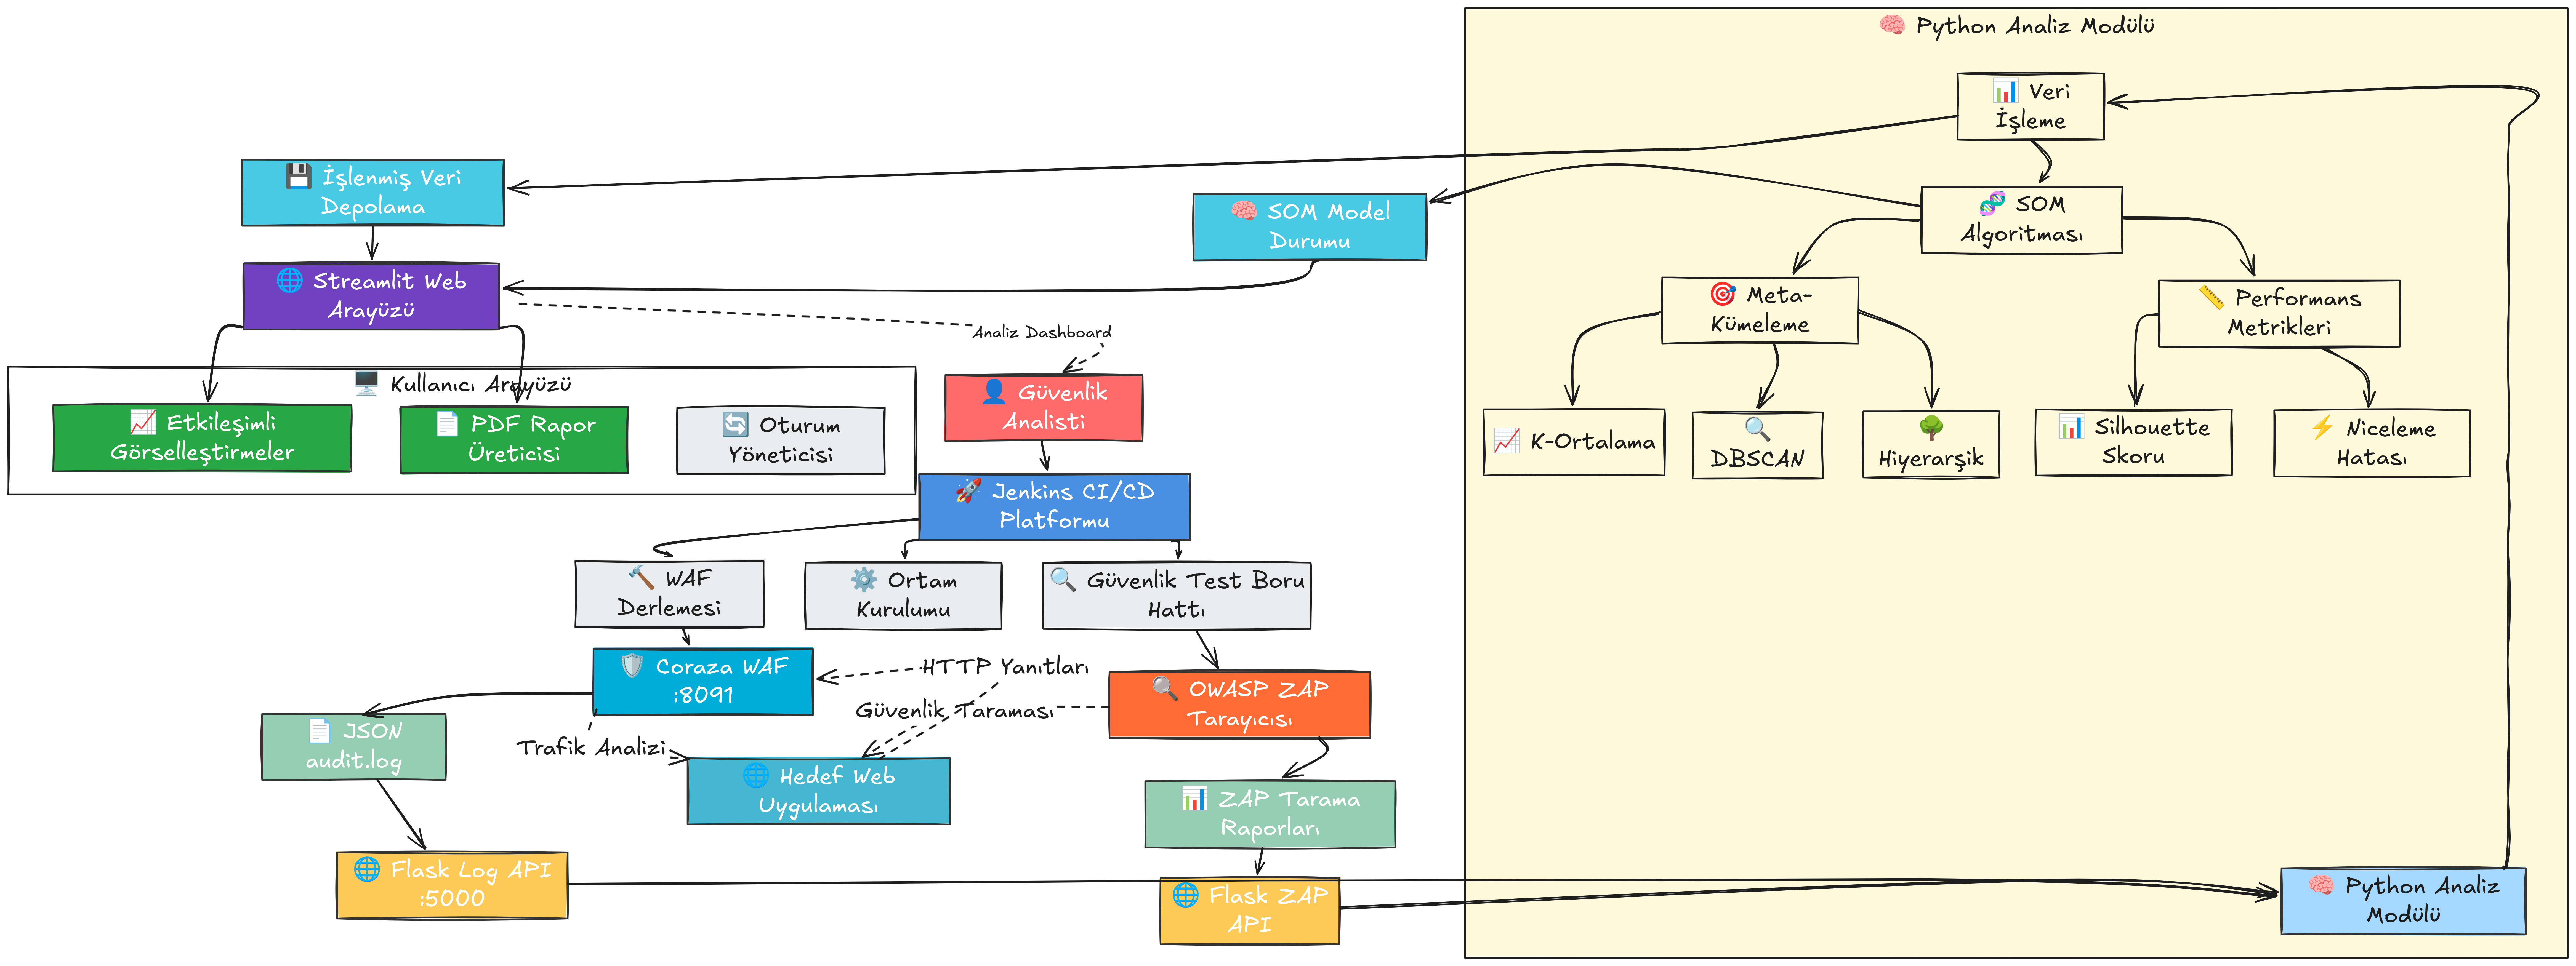
\includegraphics[width=0.95\textwidth]{images/uygulama-mimari-sablonu2.png}
    \caption{Sistem Mimarisi ve Bileşenler Arası Veri Akışı}
    \label{fig:system_architecture}
\end{figure}

Şekil \ref{fig:system_architecture}'de görüldüğü üzere, sistem güvenlik analistinin Jenkins CI/CD platformunu başlatmasıyla çalışmaya başlar. Platform, paralel olarak Coraza WAF derlemesi ve OWASP ZAP güvenlik taramasını gerçekleştirir. Hedef web uygulaması üzerindeki trafik analizi ve güvenlik taraması sonuçları, sırasıyla JSON audit logları ve ZAP raporları olarak üretilir. Bu veriler Flask API servisleri aracılığıyla Python analiz modülüne aktarılır ve SOM algoritması ile meta-kümeleme işlemlerine tabi tutulur. Son olarak, analiz sonuçları Streamlit web arayüzü üzerinden kullanıcıya sunulur.

\newpage

\subsubsection{Teknoloji Yığını Detayları}

Sistem geliştirmesinde kullanılan teknolojiler altı ana kategoride gruplandırılmıştır:

\textbf{1. Arka Uç Teknolojileri:}
\begin{itemize}
    \item \textbf{Go (v1.21):} Coraza WAF gerçekleştirimi ve yüksek başarımlı web servisi
    \item \textbf{Python (v3.8+):} Ana analiz modülü, makine öğrenmesi algoritmaları
    \item \textbf{Flask (v2.3):} REST API servisleri ve mikroservis iletişimi
\end{itemize}

\textbf{2. Makine Öğrenmesi ve Analitik:}
\begin{itemize}
    \item \textbf{MiniSom (v2.3.0):} Kendini Organize Eden Harita gerçekleştirimi \cite{minisom2017}
    \item \textbf{Scikit-learn (v1.3.0):} Üst-kümeleme algoritmaları ve başarım metrikleri
    \item \textbf{NumPy (v1.24):} Sayısal hesaplama ve dizi işlemleri
    \item \textbf{Pandas (v2.0):} Veri manipülasyonu ve JSON işleme
\end{itemize}

\textbf{3. Görselleştirme ve Ön Uç:}
\begin{itemize}
    \item \textbf{Streamlit (v1.28.0):} Etkileşimli web uygulaması çerçevesi \cite{streamlit2023}
    \item \textbf{Plotly (v5.17):} Gelişmiş veri görselleştirme ve etkileşimli grafikler \cite{plotly2015}
    \item \textbf{Matplotlib (v3.7):} İstatistiksel çizim ve grafik üretimi
\end{itemize}

\textbf{4. DevOps ve Otomasyon:}
\begin{itemize}
    \item \textbf{Jenkins (v2.414):} CI/CD boru hattı otomasyonu
    \item \textbf{Docker:} Konteynerleştirme ve dağıtım
    \item \textbf{Groovy:} Boru hattı betik dili
\end{itemize}

\textbf{5. Güvenlik ve Test:}
\begin{itemize}
    \item \textbf{OWASP ZAP (v2.14):} Güvenlik açığı tarama
    \item \textbf{OWASP CRS (v4.0):} WAF için Temel Kural Kümesi
    \item \textbf{Coraza (v3.0):} Modern WAF motoru
\end{itemize}

\newpage

\textbf{6. Veri ve Dokümantasyon:}
\begin{itemize}
    \item \textbf{JSON:} Birincil veri değişim biçimi
    \item \textbf{FPDF (v2.7):} PDF rapor üretimi
    \item \textbf{YAML:} Yapılandırma yönetimi
\end{itemize}

Her teknolojinin projeye katkısı ve seçilme nedenleri aşağıda detaylandırılmıştır.

\subsubsection{Teknolojilerin Projeye Katkıları}

\textbf{MiniSom Kütüphanesi:} Yüksek başarımlı matris işlemleri ve bellek verimli eğitim algoritmaları sağlamaktadır \cite{minisom2017}. Gauss komşuluk fonksiyonu ve dikdörtgen topoloji desteği ile günlük verilerinin topolojik eşleştirme sürecini eniyilemektedir.

\textbf{Streamlit Çerçevesi:} Hızlı prototipleme ve etkileşimli gösterge paneli geliştirme için seçilmiştir \cite{streamlit2023,ozturk2022streamlit}. Oturum durumu yönetimi, gerçek zamanlı veri güncellemeleri ve bileşen tabanlı kullanıcı etkileşimi yetenekleri, güvenlik analistlerinin sistemi etkin kullanmasını sağlamaktadır. Plotly entegrasyonu ile gelişmiş görselleştirme sağlamaktadır \cite{plotly2015}.

\textbf{Flask RESTful API:} Mikroservis mimarisi prensipleri ile günlük verisi sunumu, JSON yanıt biçimlendirmesi ve servisler arası iletişim sağlamaktadır. Jenkins boru hattı entegrasyonu için en uygun başarım sunmaktadır.

\textbf{Jenkins CI/CD Platformu:} Çoklu boru hattı düzenlemesi ve otomatik güvenlik testi için tercih edilmiştir. Groovy betikleme ile dinamik yapılandırma, paralel yürütme ve yapı yönetimi yetenekleri, sürekli güvenlik analizi iş akışını desteklemektedir. Docker konteynerleştirme teknolojisi \cite{kaplan2021docker_guvenlik} ile güvenli ve izole edilmiş çalışma ortamı sağlanmaktadır.

\textbf{Coraza WAF v3:} Go tabanlı modern mimarisi ile tam OWASP CRS uyumluluğu ve kapsamlı güvenlik izleme sağlamaktadır \cite{coraza2023}. Bellek güvenli mimari ve eşzamanlı istek işleme yetenekleri kritik avantajlar sunmaktadır.

\textbf{OWASP ZAP Tarayıcısı:} Kapsamlı saldırı benzetimi ve detaylı raporlama yetenekleri ile güvenlik testi iş akışını tamamlamaktadır \cite{zaproxy2023}.

\newpage

\textbf{Scikit-learn Kütüphanesi:} Üst-kümeleme algoritmaları ve başarım değerlendirme metrikleri için kullanılmıştır \cite{scikit_learn2011}. K-ortalama, DBSCAN, Hiyerarşik kümeleme uygulamaları ile SOM çıktısının sonraki işlemini sağlamaktadır.

\textbf{FPDF Rapor Üreticisi:} Otomatik belgeleme ve denetim izi oluşturma için tercih edilmiştir. Türkçe dil desteği, özel biçimlendirme ve gömülü grafikler ile kapsamlı güvenlik raporları üretmektedir.

\subsection{Self-Organizing Map (SOM) Algoritması}

\textbf{SOM Algoritması Nedir?}

Self-Organizing Map (SOM), yüksek boyutlu verileri düşük boyutlu (genellikle 2D) bir harita üzerinde görselleştiren ve organize eden bir yapay sinir ağı türüdür. SOM'un temel amacı, benzer özelliklere sahip verileri harita üzerinde birbirine yakın konumlarda gruplandırmaktır.

Algoritmanın çalışma prensibi:
\begin{enumerate}
    \item İki boyutlu bir nöron grid'i oluşturulur (örneğin 10x10)
    \item Her nöron, giriş verisi ile aynı boyutta bir ağırlık vektörüne sahiptir
    \item Her eğitim verisi için en benzer nöron (BMU - Best Matching Unit) bulunur
    \item BMU ve komşu nöronların ağırlıkları, giriş verisine daha benzer hale getirilir
    \item Bu işlem tüm veriler için tekrarlanır
    \item Sonuçta, benzer veriler harita üzerinde yakın bölgelerde kümelenir
\end{enumerate}

SOM'un ana avantajları:
- Yüksek boyutlu verileri görselleştirme imkanı
- Küme sayısını önceden belirleme gerektirmez
- Veri yapısını koruyan boyut indirgeme
- Anomali tespiti için kullanılabilir
- İnsan tarafından yorumlanabilir harita üretir

SOM'un dezavantajları:
- Eğitim süreci zaman alabilir
- Grid boyutunun optimize edilmesi gerekir
- Deterministik olmayan sonuçlar (rastgele başlatma nedeniyle)

\newpage

\textbf{BMU (Best Matching Unit) Seçimi:}

\textbf{BMU Nedir?}

Best Matching Unit (BMU), Türkçesi "En İyi Eşleşen Birim", SOM algoritmasının temel kavramlarından biridir. Basitçe, gelen bir veri noktasına en çok benzeyen nöronun bulunması işlemidir.

BMU'nun çalışma mantığı:
\begin{enumerate}
    \item Yeni bir veri noktası geldiğinde, SOM haritasındaki tüm nöronlar incelenir
    \item Her nöronun o veri noktasına olan "mesafesi" hesaplanır
    \item En kısa mesafeye sahip nöron "kazanan" yani BMU olarak seçilir
    \item Bu kazanan nöron ve çevresindeki komşu nöronlar güncellenir
\end{enumerate}

BMU'nun önemi:
- SOM'un öğrenme sürecinin temelini oluşturur
- Benzer verilerin harita üzerinde yakın konumlarda toplanmasını sağlar
- Her veri noktasının hangi bölgeye ait olduğunu belirler
- Anomali tespitinde kritik rol oynar (BMU mesafesi çok büyükse anomali olabilir)

\textbf{Teknik Detaylar:}

Her giriş vektörü $x(t)$ için, en küçük Öklid mesafesine sahip nöron BMU olarak seçilir:

\begin{equation}
c = \arg\min_i ||x(t) - w_i(t)||
\label{eq:bmu_selection}
\end{equation}

\textbf{SOM Güncelleme Formülü:}

\begin{equation}
w_i(t+1) = w_i(t) + \alpha(t) \cdot h_{ci}(t) \cdot [x(t) - w_i(t)]
\label{eq:som_update}
\end{equation}

Burada $\alpha(t)$ öğrenme oranı, $h_{ci}(t)$ komşuluk fonksiyonudur.

\newpage

\textbf{Quantization Error:}

\textbf{Quantization Error Nedir?}

Quantization Error (Niceleme Hatası), SOM'un ne kadar iyi eğitildiğini ölçen temel performans metrikleriuden biridir. Basitçe, her veri noktasının kendi BMU'suna olan uzaklığının ortalamasıdır.

Quantization Error'un anlamı:
\begin{enumerate}
    \item Her veri noktası için en yakın nöron (BMU) bulunur
    \item O veri noktasının BMU'ya olan mesafesi hesaplanır
    \item Tüm veri noktaları için bu mesafelerin ortalaması alınır
    \item Sonuç, SOM'un verilerimizi ne kadar iyi temsil ettiğini gösterir
\end{enumerate}

Quantization Error'un yorumlanması:
- \textbf{Düşük değer:} SOM verileri iyi temsil ediyor, nöronlar verilerine yakın
- \textbf{Yüksek değer:} SOM yetersiz, daha fazla eğitim veya farklı parametreler gerekli
- \textbf{Zaman içindeki azalma:} Eğitim ilerledikçe azalması normal ve istenen durum
- \textbf{Sabit kalma:} Eğitimin durduğunu, konverj olduğunu gösterir

Quantization Error'un kullanım alanları:
- SOM eğitiminin ne zaman duracağına karar vermek
- Farklı grid boyutlarını karşılaştırmak
- Anomali tespiti (anormal yüksek QE değerleri şüpheli)
- Model performansını değerlendirmek

\textbf{Teknik Detaylar:}

\begin{equation}
QE_{avg} = \frac{1}{N} \sum_{i=1}^{N} ||x_i - w_{BMU_i}||
\label{eq:quantization_error}
\end{equation}

\newpage

\subsubsection{Silhouette Score Hesaplama Metodolojisi}

\textbf{Silhouette Score Nedir?}

Silhouette Score, kümeleme algoritmasının ne kadar başarılı olduğunu ölçen bir metriktir. Basitçe, bir veri noktasının kendi kümesindeki diğer noktalara ne kadar yakın olduğunu ve diğer kümelerdeki noktalara ne kadar uzak olduğunu değerlendirir.

Bu metrik şu soruyu cevaplayır: "Bu nokta doğru kümede mi?" 

Silhouette Score'un çalışma prensibi:
\begin{enumerate}
    \item Her veri noktası için kendi kümesindeki diğer noktalara olan ortalama mesafesi hesaplanır (a değeri)
    \item Aynı nokta için, en yakın komşu kümedeki noktalara olan ortalama mesafe hesaplanır (b değeri)
    \item Bu iki değer karşılaştırılarak o noktanın ne kadar "doğru yerde" olduğu belirlenir
    \item Tüm noktalar için bu hesap yapılır ve ortalaması alınır
\end{enumerate}

Silhouette Score'un avantajları:
- -1 ile +1 arasında değer alır, yorumlaması kolaydır
- Küme sayısının optimal olup olmadığını gösterir
- Hem küme içi sıkılığı hem de kümeler arası ayrılığı değerlendirir
- Farklı algoritmaları karşılaştırmak için kullanılabilir

Sonuçların yorumlanması:
- +1'e yakın: Mükemmel kümeleme, noktalar doğru yerde
- 0'a yakın: Belirsiz durum, nokta küme sınırında
- -1'e yakın: Yanlış kümeleme, nokta yanlış yerde

\textbf{Teknik Detaylar:}

Silhouette Score, her bir veri noktasının kendi kümesine ne kadar iyi ait olduğunu ve diğer kümelere ne kadar benzemediğini ölçer. Bir veri noktası $i$ için silhouette katsayısı aşağıdaki formülle hesaplanır:

\begin{equation}
s(i) = \frac{b(i) - a(i)}{\max(a(i), b(i))}
\label{eq:silhouette_score}
\end{equation}

\newpage

Burada:
\begin{itemize}
    \item $a(i)$: Nokta $i$'nin kendi kümesindeki diğer noktalara olan ortalama mesafesi (küme içi mesafe)
    \item $b(i)$: Nokta $i$'nin en yakın komşu kümedeki noktalara olan ortalama mesafesi (kümeler arası mesafe)
\end{itemize}

\textbf{Matematiksel Detaylar:}

\begin{equation}
a(i) = \frac{1}{|C_I| - 1} \sum_{j \in C_I, j \neq i} d(i,j)
\label{eq:intra_cluster_distance}
\end{equation}

\begin{equation}
b(i) = \min_{J \neq I} \frac{1}{|C_J|} \sum_{j \in C_J} d(i,j)
\label{eq:inter_cluster_distance}
\end{equation}

\textbf{Silhouette Score Yorumlama:}
\begin{itemize}
    \item $s(i) \approx 1$: Nokta doğru kümeye atanmış
    \item $s(i) \approx 0$: Nokta küme sınırında 
    \item $s(i) \approx -1$: Nokta yanlış kümeye atanmış
\end{itemize}

Genel Silhouette Score, tüm noktaların silhouette katsayılarının ortalamasıdır:

\begin{equation}
\text{Silhouette Score} = \frac{1}{n} \sum_{i=1}^{n} s(i)
\label{eq:overall_silhouette}
\end{equation}

\newpage

\subsubsection{Sistem Parametreleri}

Sistemde kullanılan SOM parametreleri:

\begin{itemize}
    \item \textbf{Grid Boyutu:} $\sqrt{5 \cdot \sqrt{n}}$ (n: veri sayısı)
    \item \textbf{Sigma:} Grid boyutunun yarısı
    \item \textbf{Öğrenme Oranı:} 0.5 başlangıç değeri
    \item \textbf{İterasyon:} 1000 (kullanıcı ayarlanabilir)
\end{itemize}

\subsection{Veri Önişleme ve Analiz Stratejisi}

\subsubsection{Veri Toplama ve Doğrulama Metodolojisi}

Sistemin veri toplama süreci aşağıdaki katmanlı yapıdan oluşmaktadır:

\begin{enumerate}
    \item \textbf{Kaynak Tanımlama:} Coraza WAF \texttt{audit.log} dosyaları ve ZAP tarama sonuçları
    \item \textbf{Biçim Doğrulama:} JSON şema uyumluluğu ve yapı doğrulaması
    \item \textbf{Kalite Kontrolü:} Eksik alan tespiti, veri türü doğrulaması
    \item \textbf{Veri Temizleme:} Aykırı değer tespiti, gürültü azaltma ve veri standardizasyonu
    \item \textbf{Özellik Mühendisliği:} Alana özgü özellik çıkarımı ve normalleştirme
\end{enumerate}

\begin{figure}[!ht]
    \centering
    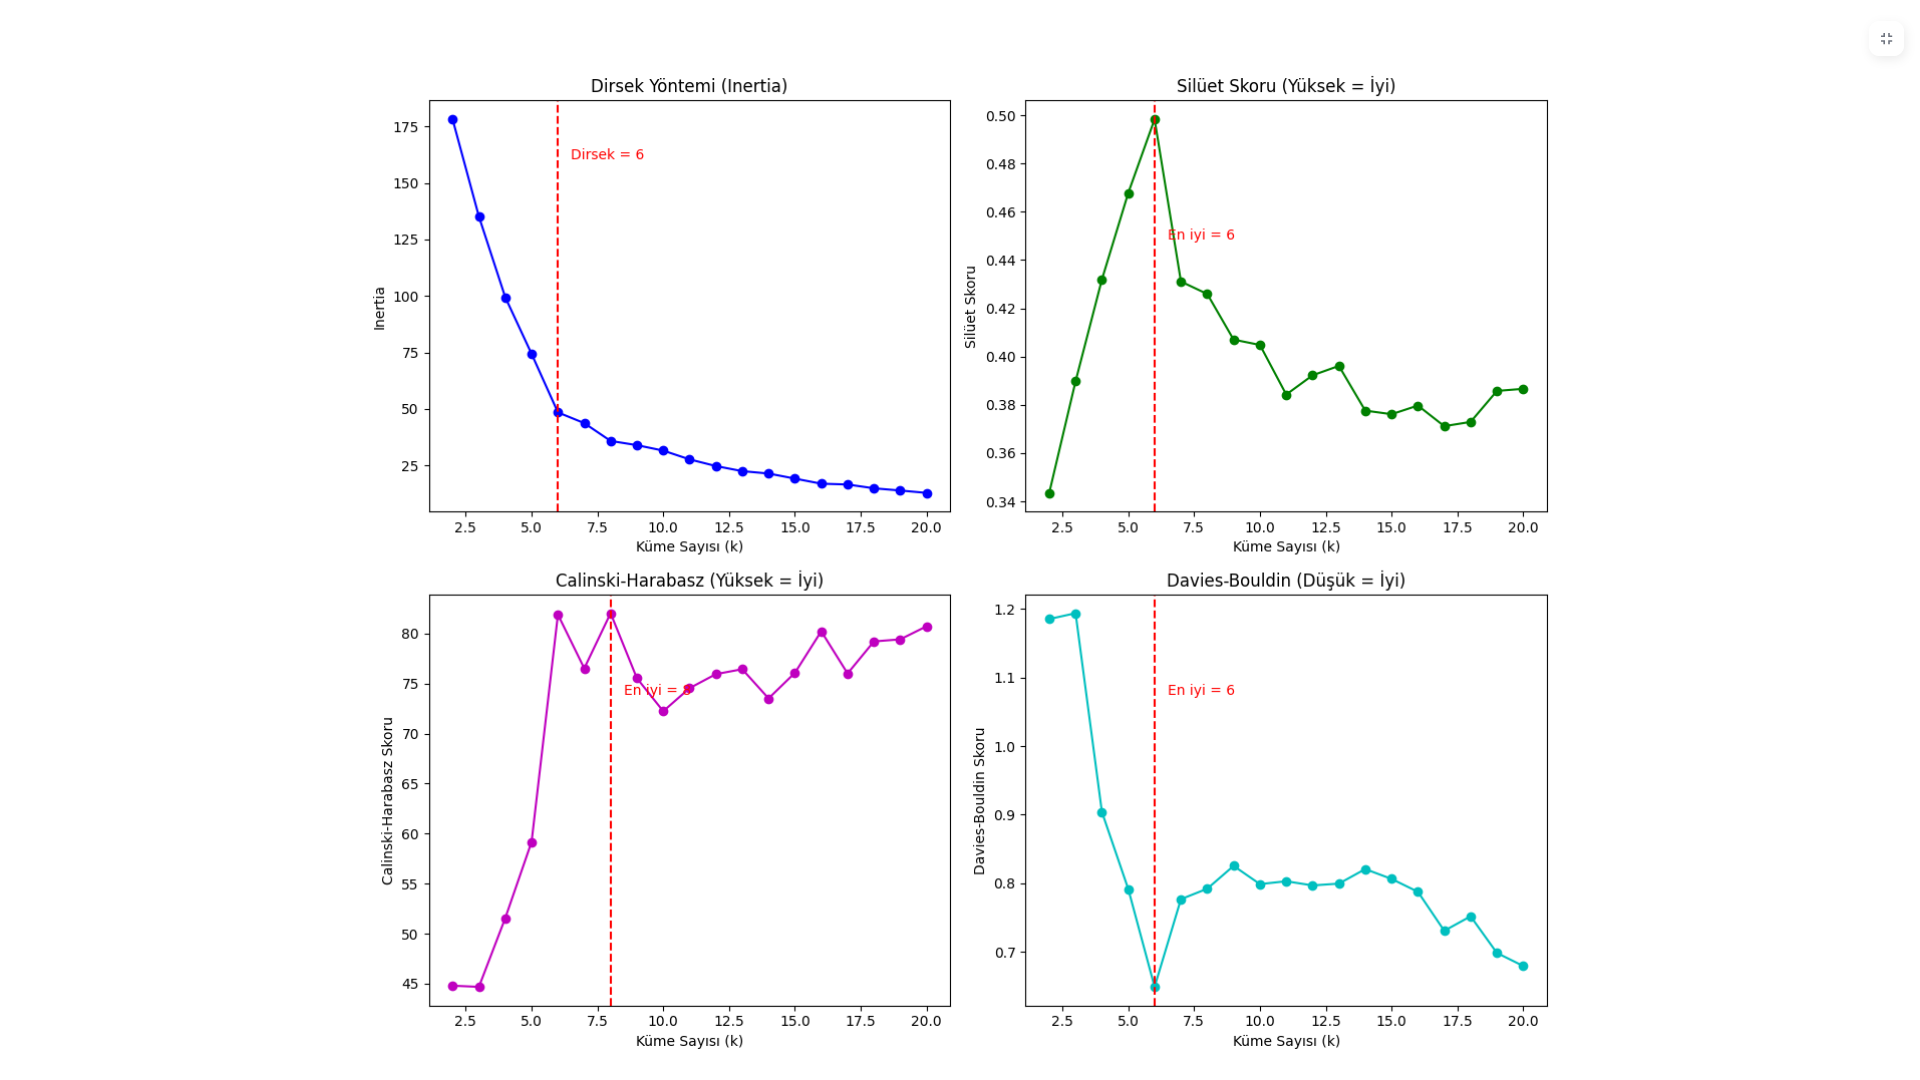
\includegraphics[width=0.8\textwidth]{images/optimal-kume-sayisi-analizi.png}
    \caption{Optimal Küme Sayısı Belirleme Analizi}
    \label{fig:optimal_clusters}
\end{figure}

Şekil \ref{fig:optimal_clusters}'de dirsek yöntemi ve silhouette analizi kullanılarak optimal küme sayısının belirlenmesi gösterilmektedir. Analiz, farklı K değerleri için WCSS (Küme İçi Kareler Toplamı) ve silhouette skoru metriklerini karşılaştırmaktadır.

\subsubsection{JSON Veri Yapısı ve İşleme}

Coraza WAF, günlük verilerini JSON biçiminde üretir \cite{coraza2023}. Sistem, iki farklı JSON yapısını destekler:

\textbf{1. İşlem Sarmalayıcı Biçimi:}
\begin{lstlisting}[language=json]
{
  "transaction": {
    "client_port": 12345,
    "request": {
      "uri": "/login",
      "method": "POST"
    },
    "timestamp": "2023-01-01T10:20:30Z",
    "is_interrupted": false
  }
}
\end{lstlisting}

\textbf{2. Düz Biçim:}
\begin{lstlisting}[language=json]
{
  "client_port": 12345,
  "request.uri": "/login", 
  "request.method": "POST",
  "timestamp": "2023-01-01T10:20:30Z",
  "is_interrupted": false
}
\end{lstlisting}

\newpage

\subsubsection{Analiz Stratejisi}

Sistem, uyarlanabilir analiz stratejisi kullanarak farklı veri kümeleri için en uygun analiz yaklaşımını belirler:

\textbf{Sıralı Analiz Aşamaları:}

\begin{enumerate}
    \item \textbf{Keşifsel Veri Analizi:} Veri dağılımı, bağıntı analizi
    \item \textbf{Özellik Seçimi:} Varyans eşiği, bağıntı filtreleme
    \item \textbf{SOM Eğitimi:} Izgara optimizasyonu, parametre ayarlama
    \item \textbf{Üst-Kümeleme:} Algoritma seçimi, doğrulama metrikleri
\end{enumerate}

\textbf{Duruma Özgü Analiz Seçimi:}

\begin{itemize}
    \item \textbf{Küçük Veri Kümeleri (n < 1000):} Doğrudan SOM eğitimi, basit görselleştirme
    \item \textbf{Orta Boyut Kümeler (1000 < n < 10000):} Toplu işleme, üst-kümeleme
    \item \textbf{Büyük Veri Kümeleri (n > 10000):} Artımlı öğrenme, dağıtık işleme
\end{itemize}

\textbf{Başarım Metriklerinin Seçim Ölçütleri:}

\begin{table}[!ht]
\centering
\caption{Analiz Metriklerinin Kullanım Alanları}
\label{tab:metrics_usage}
\begin{tabular}{|l|p{0.3\textwidth}|p{0.4\textwidth}|}
\hline
\textbf{Metrik} & \textbf{Kullanım Alanı} & \textbf{Avantajlar} \\
\hline
Silhouette Skoru & Küme kalitesi değerlendirme & Küme sıkılığı ve ayrılık ölçümü \\
\hline
Calinski-Harabasz & Optimal küme sayısı belirleme & Varyans oranı analizi \\
\hline
Davies-Bouldin & Küme kompaktlığı analizi & Düşük değerler iyi kümelemeyi gösterir \\
\hline
Niceleme Hatası & SOM temsil kalitesi & Eğitim yakınsama izleme \\
\hline
Topolojik Hata & Komşuluk korunması & Topoloji koruma değerlendirmesi \\
\hline
\end{tabular}
\end{table}

\newpage

\subsubsection{Calinski-Harabasz İndeksi}

\textbf{Calinski-Harabasz İndeksi Nedir?}

Calinski-Harabasz (CH) İndeksi, kümeleme kalitesini değerlendiren ve optimal küme sayısını bulmak için kullanılan bir metriktir. Bu indeks, kümeler arası ayrılık ile küme içi sıkılık oranını hesaplar.

CH İndeksinin çalışma prensibi:
\begin{enumerate}
    \item Kümeler arası varyans hesaplanır
    \item Küme içi varyans hesaplanır  
    \item Bu iki değerin oranı alınır ve serbestlik derecelerine göre düzeltilir
    \item Yüksek değer daha iyi kümelenme anlamına gelir
\end{enumerate}

CH İndeksinin avantajları:
- Optimal küme sayısını belirlemede etkili
- Hesaplama hızı yüksek
- Farklı küme şekilleri için genel olarak güvenilir
- Küme sayısı arttıkça nasıl değiştiğini takip etmek kolay

CH İndeksinin yorumlanması:
- \textbf{Yüksek değer:} İyi kümelenme, kümeler birbirinden ayrık ve içten sıkı
- \textbf{Düşük değer:} Zayıf kümelenme, kümeler belirsiz
- \textbf{Maksimum nokta:} Genellikle optimal küme sayısını gösterir

\textbf{Teknik Detaylar:}

\begin{equation}
CH = \frac{SS_B / (k-1)}{SS_W / (n-k)}
\label{eq:calinski_harabasz}
\end{equation}

Burada:
\begin{itemize}
    \item $SS_B$: Kümeler arası kareler toplamı
    \item $SS_W$: Küme içi kareler toplamı
    \item $k$: Küme sayısı
    \item $n$: Toplam veri noktası sayısı
\end{itemize}

\newpage

\subsubsection{Davies-Bouldin İndeksi}

\textbf{Davies-Bouldin İndeksi Nedir?}

Davies-Bouldin (DB) İndeksi, kümeleme kalitesini ölçen ve Calinski-Harabasz'ın tersine düşük değerlerin iyi olduğu bir metriktir. Her kümenin kendi içindeki dağılım ile en yakın komşu kümeye olan mesafesini karşılaştırır.

DB İndeksinin çalışma prensibi:
\begin{enumerate}
    \item Her küme için içindeki noktaların merkeze olan ortalama mesafesi hesaplanır
    \item Her küme için diğer küme merkezlerine olan mesafeler bulunur
    \item Her küme çifti için benzerlik oranı hesaplanır
    \item En kötü (en yüksek) benzerlik oranları toplanır ve ortalaması alınır
\end{enumerate}

DB İndeksinin avantajları:
- Küme kompaktlığını ve ayrılığını birlikte değerlendirir
- Hesaplama basit ve hızlı
- Küme şekillerinden görece bağımsız
- Optimal küme sayısını belirlemede kullanışlı

DB İndeksinin yorumlanması:
- \textbf{Düşük değer (0'a yakın):} Mükemmel kümelenme, kompakt ve ayrık kümeler
- \textbf{Yüksek değer:} Zayıf kümelenme, kümeler iç içe veya dağınık
- \textbf{Minimum nokta:} Optimal küme sayısını gösterir

\textbf{Teknik Detaylar:}

\begin{equation}
DB = \frac{1}{k} \sum_{i=1}^{k} \max_{j \neq i} \left( \frac{\sigma_i + \sigma_j}{d(c_i, c_j)} \right)
\label{eq:davies_bouldin}
\end{equation}

Burada:
\begin{itemize}
    \item $\sigma_i$: Küme $i$'nin içindeki noktaların merkeze olan ortalama mesafesi
    \item $d(c_i, c_j)$: Küme $i$ ve $j$ merkezleri arasındaki mesafe
    \item $k$: Küme sayısı
\end{itemize}

\newpage

\subsubsection{Topological Error}

\textbf{Topological Error Nedir?}

Topological Error (Topolojik Hata), SOM'un giriş verilerinin komşuluk ilişkilerini ne kadar iyi koruduğunu ölçen bir metriktir. SOM'un temel özelliklerinden biri olan "topology preservation" yeteneğini değerlendirir.

Topological Error'un çalışma prensibi:
\begin{enumerate}
    \item Her veri noktası için BMU (en yakın nöron) bulunur
    \item Aynı veri noktası için ikinci en yakın nöron belirlenir
    \item BMU ile ikinci en yakın nöronun SOM haritasında komşu olup olmadığı kontrol edilir
    \item Komşu değillerse, bu bir topolojik hata sayılır
    \item Tüm hatalar toplanır ve toplam veri sayısına bölünür
\end{enumerate}

Topological Error'un önemi:
- SOM'un topoloji koruma yeteneğini doğrular
- Düşük değer, SOM'un giriş uzayının yapısını iyi koruduğunu gösterir
- Grid boyutunun ve parametrelerin uygunluğunu değerlendirir
- Görselleştirme kalitesinin göstergesidir

Topological Error'un yorumlanması:
- \textbf{Düşük değer (0'a yakın):} Mükemmel topoloji korunması
- \textbf{Yüksek değer:} Topoloji bozulması, SOM parametreleri gözden geçirilmeli
- \textbf{0 değeri:} İdeal durum, tüm komşuluklar korunmuş

\textbf{Teknik Detaylar:}

\begin{equation}
TE = \frac{1}{N} \sum_{i=1}^{N} u(x_i)
\label{eq:topological_error}
\end{equation}

Burada:
\begin{equation}
u(x_i) = \begin{cases}
1 & \text{eğer BMU ve 2. BMU komşu değilse} \\
0 & \text{eğer BMU ve 2. BMU komşuysa}
\end{cases}
\label{eq:topological_error_function}
\end{equation}

\newpage

\subsection{Meta-Kümeleme Algoritmaları}

Sistem, SOM çıktısı üzerinde farklı kümeleme algoritmalarını uygular:

\subsubsection{K-Means Clustering}

\textbf{K-Means Algoritması Nedir?}

K-Means, veri setindeki noktaları önceden belirlenen sayıda (k) gruba ayıran bir kümeleme algoritmasıdır. Algoritmanın temel amacı, her bir veri noktasını en yakın küme merkezine atayarak, küme içi benzerliği maksimize etmek ve kümeler arası farklılığı artırmaktır.

Algoritma şu adımları takip eder:
\begin{enumerate}
    \item Küme sayısı (k) önceden belirlenir
    \item K adet merkez nokta rastgele yerleştirilir
    \item Her veri noktası, en yakın merkez noktaya atanır
    \item Her kümenin yeni merkez noktası, o kümedeki tüm noktaların ortalaması alınarak hesaplanır
    \item Merkez noktalar değişmeyene kadar 3. ve 4. adımlar tekrarlanır
\end{enumerate}

K-Means'in ana avantajı hesaplama hızı ve basitliğidir. Ancak küme sayısının önceden bilinmesi gerekir ve küresel olmayan küme şekillerinde başarısız olabilir.

\textbf{Teknik Detaylar:}

\begin{equation}
J = \sum_{i=1}^{k} \sum_{x \in C_i} ||x - \mu_i||^2
\label{eq:kmeans_objective}
\end{equation}

Burada $\mu_i$ küme merkezleridir.

\newpage

\subsubsection{DBSCAN Algorithm}

\textbf{DBSCAN Algoritması Nedir?}

DBSCAN (Density-Based Spatial Clustering of Applications with Noise), veri yoğunluğuna dayalı olarak kümeleme yapan bir algoritmadır. K-Means'ten farklı olarak, küme sayısını önceden belirleme gerektirmez ve keyfi şekillerdeki kümeleri tespit edebilir.

Algoritmanın temel prensibi, belirli bir yarıçap içerisinde yeterli sayıda komşuya sahip noktaları "yoğun bölgeler" olarak tanımlamak ve bu bölgeleri genişleterek kümeleri oluşturmaktır. Yeterli komşuya sahip olmayan noktalar ise gürültü (noise) olarak sınıflandırılır.

DBSCAN'in çalışma mantığı:
\begin{enumerate}
    \item Her veri noktası için epsilon ($\varepsilon$) yarıçapındaki komşu sayısı hesaplanır
    \item Eğer bir nokta minimum nokta sayısından (MinPts) fazla komşuya sahipse "çekirdek nokta" olur
    \item Çekirdek noktalardan başlayarak, komşu noktalar aynı kümeye dahil edilir
    \item Bu işlem tüm erişilebilir noktalar kümeye dahil edilene kadar devam eder
    \item Hiçbir kümeye dahil olmayan noktalar gürültü olarak işaretlenir
\end{enumerate}

DBSCAN'in ana avantajları:
- Küme sayısını önceden belirleme gerektirmez
- Keyfi şekillerdeki kümeleri bulabilir
- Gürültü noktalarını otomatik tespit eder
- Farklı yoğunluktaki kümeleri işleyebilir

\textbf{Teknik Detaylar:}

DBSCAN (Density-Based Spatial Clustering of Applications with Noise), yoğunluk tabanlı kümeleme algoritmasıdır. İki temel parametre kullanır: $\epsilon$ (komşuluk yarıçapı) ve $MinPts$ (minimum nokta sayısı).

\newpage

\textbf{Temel Tanımlar:}

\textbf{1. $\epsilon$-Neighborhood (Epsilon Komşuluğu):}
Bir nokta $p$'nin $\epsilon$-komşuluğu aşağıdaki şekilde tanımlanır:

\begin{equation}
N_{\epsilon}(p) = \{q \in D | \text{dist}(p,q) \leq \epsilon\}
\label{eq:epsilon_neighborhood}
\end{equation}

\textbf{2. Core Point (Çekirdek Nokta):}
Bir nokta $p$, eğer $|N_{\epsilon}(p)| \geq MinPts$ koşulunu sağlıyorsa core point'tir.

\begin{equation}
\text{CorePoint}(p) = |N_{\epsilon}(p)| \geq MinPts
\label{eq:core_point}
\end{equation}

\textbf{3. Border Point (Sınır Nokta):}
Bir nokta $p$, core point değilse ancak en az bir core point'in $\epsilon$-komşuluğunda yer alıyorsa border point'tir.

\textbf{4. Noise Point (Gürültü Nokta):}
Ne core point ne de border point olan noktalar noise point olarak sınıflandırılır.

\textbf{Yoğunluk Bağlantısı (Density Connectivity):}

\textbf{Directly Density-Reachable:}
Nokta $q$, nokta $p$'den directly density-reachable'dır eğer:
\begin{itemize}
    \item $q \in N_{\epsilon}(p)$ ve
    \item $p$ bir core point ise
\end{itemize}

\textbf{Density-Reachable:}
Nokta $q$, nokta $p$'den density-reachable'dır eğer $p_1, p_2, ..., p_n$ nokta zinciri mevcutsa:
$p_1 = p$, $p_n = q$ ve her $p_{i+1}$ nokta $p_i$'den directly density-reachable'dır.

\textbf{Density-Connected:}
İki nokta $p$ ve $q$ density-connected'dır eğer bir $o$ noktası mevcutsa hem $p$ hem de $q$ bu noktadan density-reachable'dır.

\newpage

\textbf{DBSCAN Parametre Seçimi:}

\begin{itemize}
    \item \textbf{$\epsilon$ Belirleme:} K-distance grafik metoduyla optimal $\epsilon$ değeri bulunur
    \item \textbf{MinPts Seçimi:} Genellikle $MinPts = 2 \times \text{boyut}$ kuralı kullanılır
    \item \textbf{Sistemde Kullanılan Değerler:} $\epsilon = 0.5$, $MinPts = 5$
\end{itemize}

\textbf{DBSCAN Avantajları:}
\begin{itemize}
    \item Küme sayısını önceden belirleme gerektirmez
    \item Gürültü noktalarını otomatik tespit eder
    \item Keyfi şekilli kümeleri bulabilir
    \item Outlier detection capability'si
\end{itemize}

\subsubsection{Hierarchical Clustering}

\textbf{Hiyerarşik Kümeleme Nedir?}

Hiyerarşik kümeleme, veri noktaları arasındaki mesafe ilişkilerini kullanarak ağaç benzeri (dendrogram) bir küme yapısı oluşturan algoritmadır. Bu algoritma, farklı küme sayıları için sonuçları aynı anda görebilme avantajı sağlar.

İki ana türü vardır:

\textbf{1. Aglomeratif (Agglomerative) Kümeleme:}
- Alt-yukarı (bottom-up) yaklaşım kullanır
- Her veri noktası kendi kümesi olarak başlar
- En yakın kümeleri tekrar tekrar birleştirerek büyük kümeler oluşturur
- Tüm noktalar tek kümede toplanana kadar devam eder

\textbf{2. Bölen (Divisive) Kümeleme:}
- Yukarı-alt (top-down) yaklaşım kullanır
- Tüm veriler tek kümede başlar
- En uzak alt grupları ayırarak küçük kümeler oluşturur
- Her nokta kendi kümesinde kalana kadar devam eder

Hiyerarşik kümelemenin ana avantajları:
- Dendrogram ile küme yapısının görselleştirilmesi
- Farklı küme sayıları için sonuçların eş zamanlı elde edilmesi
- Deterministik sonuçlar (rastgelelik yok)
- Küme sayısını önceden belirleme gerektirmez

\newpage

Ana dezavantajı, büyük veri setlerinde yüksek hesaplama maliyetidir (O(n³)).

\textbf{Teknik Detaylar:}

Linkage criteria için üç farklı yöntem desteklenir:

\begin{itemize}
    \item \textbf{Single Linkage:} $d(C_i, C_j) = \min_{x \in C_i, y \in C_j} d(x,y)$
    \item \textbf{Complete Linkage:} $d(C_i, C_j) = \max_{x \in C_i, y \in C_j} d(x,y)$
    \item \textbf{Average Linkage:} $d(C_i, C_j) = \frac{1}{|C_i||C_j|} \sum_{x \in C_i} \sum_{y \in C_j} d(x,y)$
\end{itemize}

\subsection{Boyut İndirgeme Teknikleri}

\subsubsection{Principal Component Analysis (PCA)}

PCA, varyansı maksimize eden linear transformation kullanır:

\begin{equation}
Y = XW
\label{eq:pca_transform}
\end{equation}

Burada $W$ eigenvector matrix'idir.

\subsubsection{t-SNE (t-Distributed Stochastic Neighbor Embedding)}

t-SNE, yüksek boyutlu benzerlik dağılımını düşük boyutta korur:

\begin{equation}
C = \sum_i \sum_j p_{ij} \log \frac{p_{ij}}{q_{ij}}
\label{eq:tsne_cost}
\end{equation}

\newpage

\subsubsection{UMAP (Uniform Manifold Approximation and Projection)}

UMAP, manifold structure'ı koruyarak boyut indirgeme yapar:

\begin{table}[!ht]
\centering
\caption{Boyut İndirgeme Tekniklerinin Karşılaştırması}
\label{tab:dim_reduction_comparison}
\begin{tabular}{|l|c|c|c|c|}
\hline
\textbf{Teknik} & \textbf{Lineer} & \textbf{Hız} & \textbf{Global Yapı} & \textbf{Local Yapı} \\
\hline
PCA & Evet & Çok Hızlı & İyi & Zayıf \\
\hline
t-SNE & Hayır & Yavaş & Zayıf & Mükemmel \\
\hline
UMAP & Hayır & Hızlı & İyi & İyi \\
\hline
\end{tabular}
\end{table}

\subsection{Sistem Mimarisi Detayları}

\subsubsection{Flask API Servisleri}

Sistem, mikroservis mimarisi ile iki farklı Flask API servisi kullanır:

\textbf{Flask Log API (Port 5000):}

Jenkins pipeline içerisinde dinamik olarak oluşturulan Flask uygulaması:

\begin{lstlisting}[language=python]
from flask import Flask, jsonify
import json, os

app = Flask(__name__)
LOG_PATH = "./coraza/reports/audit.log"

@app.route('/logs', methods=['GET'])
def get_logs():
    logs = []
    with open(LOG_PATH, 'r') as f:
        for line in f:
            try:
                logs.append(json.loads(line.strip()))
            except json.JSONDecodeError:
                continue
    return jsonify(logs)

if __name__ == '__main__':
    app.run(host='0.0.0.0', port=5000)
\end{lstlisting}

\newpage

\subsubsection{Veri Akışı ve Sistem Entegrasyonu}

Sistem veri akışı şu şekilde çalışır:

\begin{enumerate}
    \item \textbf{Boru Hattı Başlatma:} CorazaWAF-Log-Last boru hattı başlatılır
    \item \textbf{Ortam Kurulumu:} Go, Flask kurulumu ve bağımlılık yönetimi
    \item \textbf{WAF Derleme:} Coraza WAF v3 ikili dosya derleme
    \item \textbf{Servis Başlatma:} WAF port 8091, Flask API port 5000'de başlatılır
    \item \textbf{Güvenlik Tarama:} ZAP tarayıcısı hedef URL'yi tarar
    \item \textbf{Log Üretimi:} WAF JSON \texttt{audit.log} üretir
    \item \textbf{Veri Analizi:} Streamlit modülü API'den veri alır ve işler
\end{enumerate}

\subsection{Validasyon ve Güvenilirlik Stratejileri}

\subsubsection{Çapraz Doğrulama Metodolojisi}

\begin{itemize}
    \item \textbf{K-Katlı Çapraz Doğrulama:} SOM parametre optimizasyonu
    \item \textbf{Bootstrap Örnekleme:} Güven aralıkları hesaplama  
    \item \textbf{Permütasyon Testi:} İstatistiksel anlamlılık testi
    \item \textbf{Kararlılık Analizi:} Kümeleme tutarlılığı değerlendirmesi
\end{itemize}

\subsubsection{Performans İzleme}

Sistem performansı sürekli izlenir:

\begin{itemize}
    \item \textbf{Bellek Kullanımı:} Gerçek zamanlı RAM izleme
    \item \textbf{İşleme Süresi:} Algoritma yürütme takibi
    \item \textbf{Doğruluk Metrikleri:} Kümeleme kalitesi değerlendirmesi
    \item \textbf{Hata Oranları:} Sistem arıza tespiti
\end{itemize}

Bu kapsamlı metodoloji, sistemin güvenilir ve ölçeklenebilir bir şekilde çalışmasını sağlamaktadır.












\section{UYGULAMA}

Bu bölümde, Coraza WAF log analizi ve SOM kümeleme sisteminin implementasyonu, sistem bileşenlerinin entegrasyonu ve gerçekleştirilen testler detaylı olarak açıklanmaktadır.

\subsection{Sistem Geliştirme Süreci}

Proje, Agile metodoloji kullanılarak aşamalı olarak geliştirilmiştir. Geliştirme süreci üç ana aşamadan oluşmaktadır:

\begin{enumerate}
    \item \textbf{Altyapı Kurulumu:} Jenkins, Coraza WAF ve OWASP ZAP entegrasyonu
    \item \textbf{Analiz Modülü Geliştirme:} Python tabanlı SOM analiz sistemi
    \item \textbf{Web Arayüzü Geliştirme:} Streamlit ile kullanıcı arayüzü
\end{enumerate}

\subsection{Jenkins CI/CD Boru Hattı Uygulaması}

Sistem, iki ana Jenkins boru hattı kullanmaktadır. Ana boru hattı (CorazaWAF-Log-Last) aşağıdaki temel aşamaları içermektedir:

\subsubsection{Ortam Hazırlama ve Bağımlılık Yönetimi}

Boru hattı öncelikle gerekli bağımlılıkları kurar: Python3, \texttt{pip}, Flask ve \texttt{wget} paketleri \texttt{apt} paket yöneticisi ile sisteme yüklenir.

\textbf{Go Sürüm Yönetimi:}
\begin{lstlisting}[language=bash]
LATEST_GO=$(curl -s https://go.dev/VERSION?m=text)
wget https://golang.org/dl/${LATEST_GO}.linux-amd64.tar.gz
sudo tar -C /usr/local -xzf ${LATEST_GO}.linux-amd64.tar.gz
export PATH=$PATH:/usr/local/go/bin
\end{lstlisting}

\subsubsection{Dinamik Servis Oluşturma}

Boru hattı, \texttt{writeFile} direktifi ile dinamik Flask uygulaması oluşturur ve Go tabanlı WAF'ı arka planda çalıştırır. Her iki servis de paralel olarak 8091 ve 8080 portlarında hizmet verir.

\newpage

\begin{figure}[!ht]
    \centering
    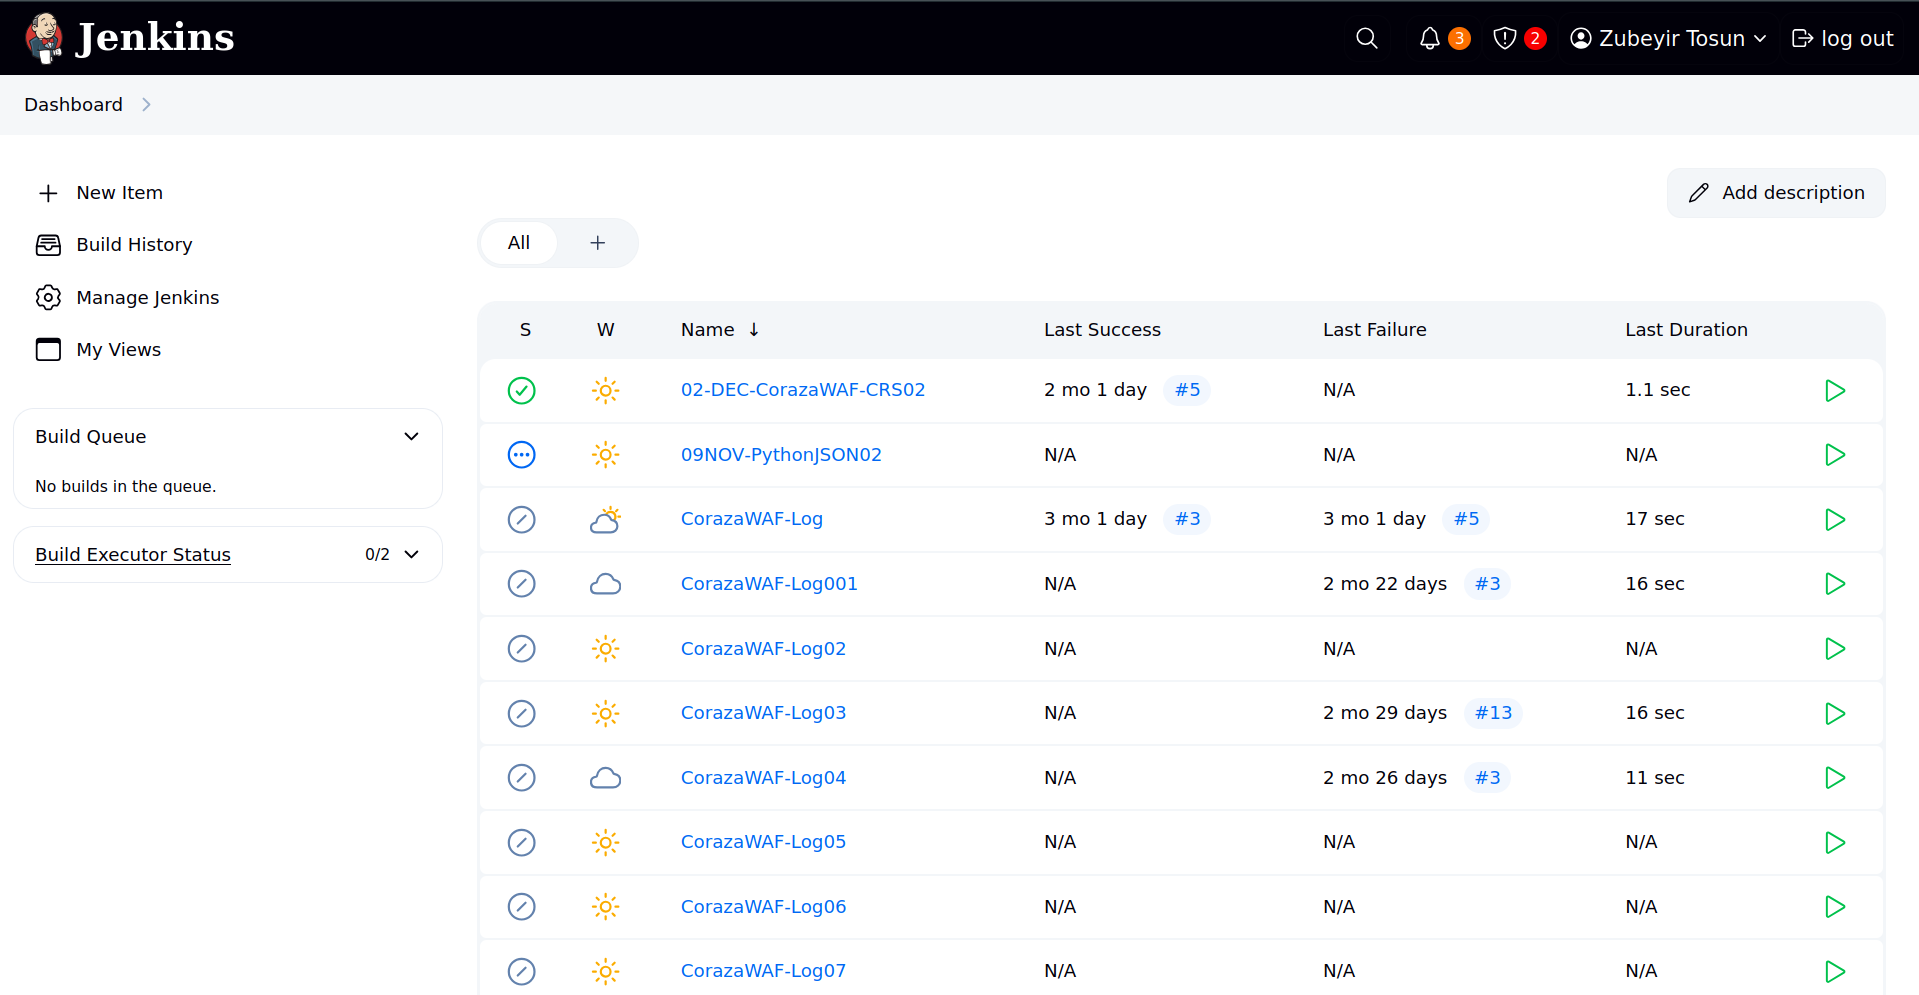
\includegraphics[width=0.8\textwidth]{images/jenkins-dashboard.png}
    \caption{Jenkins Pipeline Dashboard Görünümü}
    \label{fig:jenkins_dashboard}
\end{figure}

Boru hattı çalıştırıldığında, Şekil \ref{fig:jenkins_dashboard}'de görüldüğü gibi Jenkins gösterge paneli üzerinden tüm aşamaların durumu izlenebilmektedir. Gösterge paneli, her boru hattının başarı durumunu, çalışma süresini ve log çıktılarını gerçek zamanlı olarak göstermektedir.

\subsubsection{Çoklu Boru Hattı Yönetimi}

Sistem, dört farklı boru hattı ile tam otomatik dağıtım sağlar:

\begin{itemize}
    \item \textbf{CorazaWAF-Log-Last:} Ana WAF log toplama ve analiz boru hattı
    \item \textbf{Flask-API-Server:} RESTful API servisi
    \item \textbf{ZAP-Security-Scanner:} Otomatik güvenlik tarama modülü
    \item \textbf{Streamlit-Analytics:} Web tabanlı analiz arayüzü
\end{itemize}

Her boru hattı, kendi sorumluluk alanında bağımsız çalışır ve sonuçlarının merkezi bir gösterge paneli üzerinden raporlar.

\subsubsection{Coraza WAF Konfigürasyonu}

Coraza WAF, Jenkins container içerisinde Go programı olarak çalıştırılmaktadır. WAF konfigürasyonu aşağıdaki direktiflerle yapılır:

\begin{lstlisting}[language=go]
// WAF yapılandırması
directives := `SecRuleEngine On
Include etc/crs4/crs-setup.conf
Include etc/crs4/rules/*.conf
SecAction "id:900110,phase:1,pass,nolog,setvar:tx.inbound_anomaly_score_threshold=5,setvar:tx.outbound_anomaly_score_threshold=4"
SecRule REQUEST_URI "@streq /test" "id:1000,phase:1,deny,status:403"
SecRequestBodyLimit 13107200
SecResponseBodyLimit 524288
SecAuditLog ./reports/audit.log
SecAuditLogFormat JSON
SecDebugLog ./reports/debug.log
SecDebugLogLevel 9`

config := coraza.NewWAFConfig().
    WithDirectives(directives).
    WithRootFS(os.DirFS("/"))

waf, err := coraza.NewWAF(config)
\end{lstlisting}

WAF, Jenkins sunucusuna (\texttt{http://jenkins:8080}) yönlendirme yapan ters vekil sunucu olarak port 8091'de çalışır.

\subsubsection{ZAP Tarayıcı Boru Hattı}

OWASP ZAP güvenlik taraması için ayrı bir boru hattı kullanılır. Ana işlem adımları:

\textbf{Hedef Tanımlama:}
Hedef URL (\texttt{http://172.19.0.4:8091}) ve ZAP API uç noktaları (\texttt{zapscanner:8090}) tanımlanır.

\begin{lstlisting}[language=bash]
curl -X GET "http://$ZAP_HOST:$ZAP_PORT/JSON/core/action/accessUrl/?url=${TARGET_URL}"
curl -X GET "http://$ZAP_HOST:$ZAP_PORT/JSON/ascan/action/scan/?url=${TARGET_URL}"
\end{lstlisting}

\newpage

\subsection{Python Analiz Modülü}

Analiz modülü, beş ana Python dosyasından oluşmaktadır:

\begin{itemize}
    \item \textbf{main.py:} Ana uygulama ve Streamlit arayüzü
    \item \textbf{data\_processing.py:} Veri önişleme ve SOM eğitimi
    \item \textbf{visualizations.py:} Görselleştirme ve analiz sonuçları
    \item \textbf{advanced\_analysis.py:} Gelişmiş analiz yöntemleri
    \item \textbf{pdf\_report.py:} PDF rapor üretimi
\end{itemize}

\subsubsection{Veri Önişleme Modülü}

Veri önişleme modülü, JSON log dosyalarını SOM algoritması için uygun formata dönüştürür:

\begin{lstlisting}[language=python]
def preprocess_data(df, missing_method, uri_threshold=10):
    # Zorunlu sütun kontrolü
    required_columns = [
        'transaction.client_port',
        'transaction.request.uri',
        'transaction.timestamp',
        'transaction.is_interrupted',
        'transaction.request.method'
    ]
    
    # Eksik sütunlar için varsayılan değerler
    for col in required_columns:
        if col not in df.columns:
            df[col] = get_default_value(col)
    
    # Özellik çıkarımı
    df = create_features(df, uri_threshold)
    X = prepare_final_features(df)
    
    return df, X
\end{lstlisting}

\newpage

\subsubsection{SOM Eğitim Modülü}

SOM algoritması, MiniSom kütüphanesi kullanılarak implementa edilmiştir:

\begin{lstlisting}[language=python]
def train_som(X, grid_size, sigma, learning_rate, iterations):
    # SOM modeli oluşturma
    som = MiniSom(grid_size, grid_size, X.shape[1], 
                  sigma=sigma, learning_rate=learning_rate,
                  neighborhood_function='gaussian',
                  topology='rectangular')
    
    # Ağırlıkları rastgele başlatma
    som.random_weights_init(X)
    
    # Eğitim süreci
    som.train(X, iterations, verbose=True)
    
    return som
\end{lstlisting}

\subsection{Streamlit Web Arayüzü}

Web arayüzü, kullanıcı dostu bir deneyim sunmak için Streamlit çerçevesi kullanılarak geliştirilmiştir.

\begin{figure}[!ht]
    \centering
    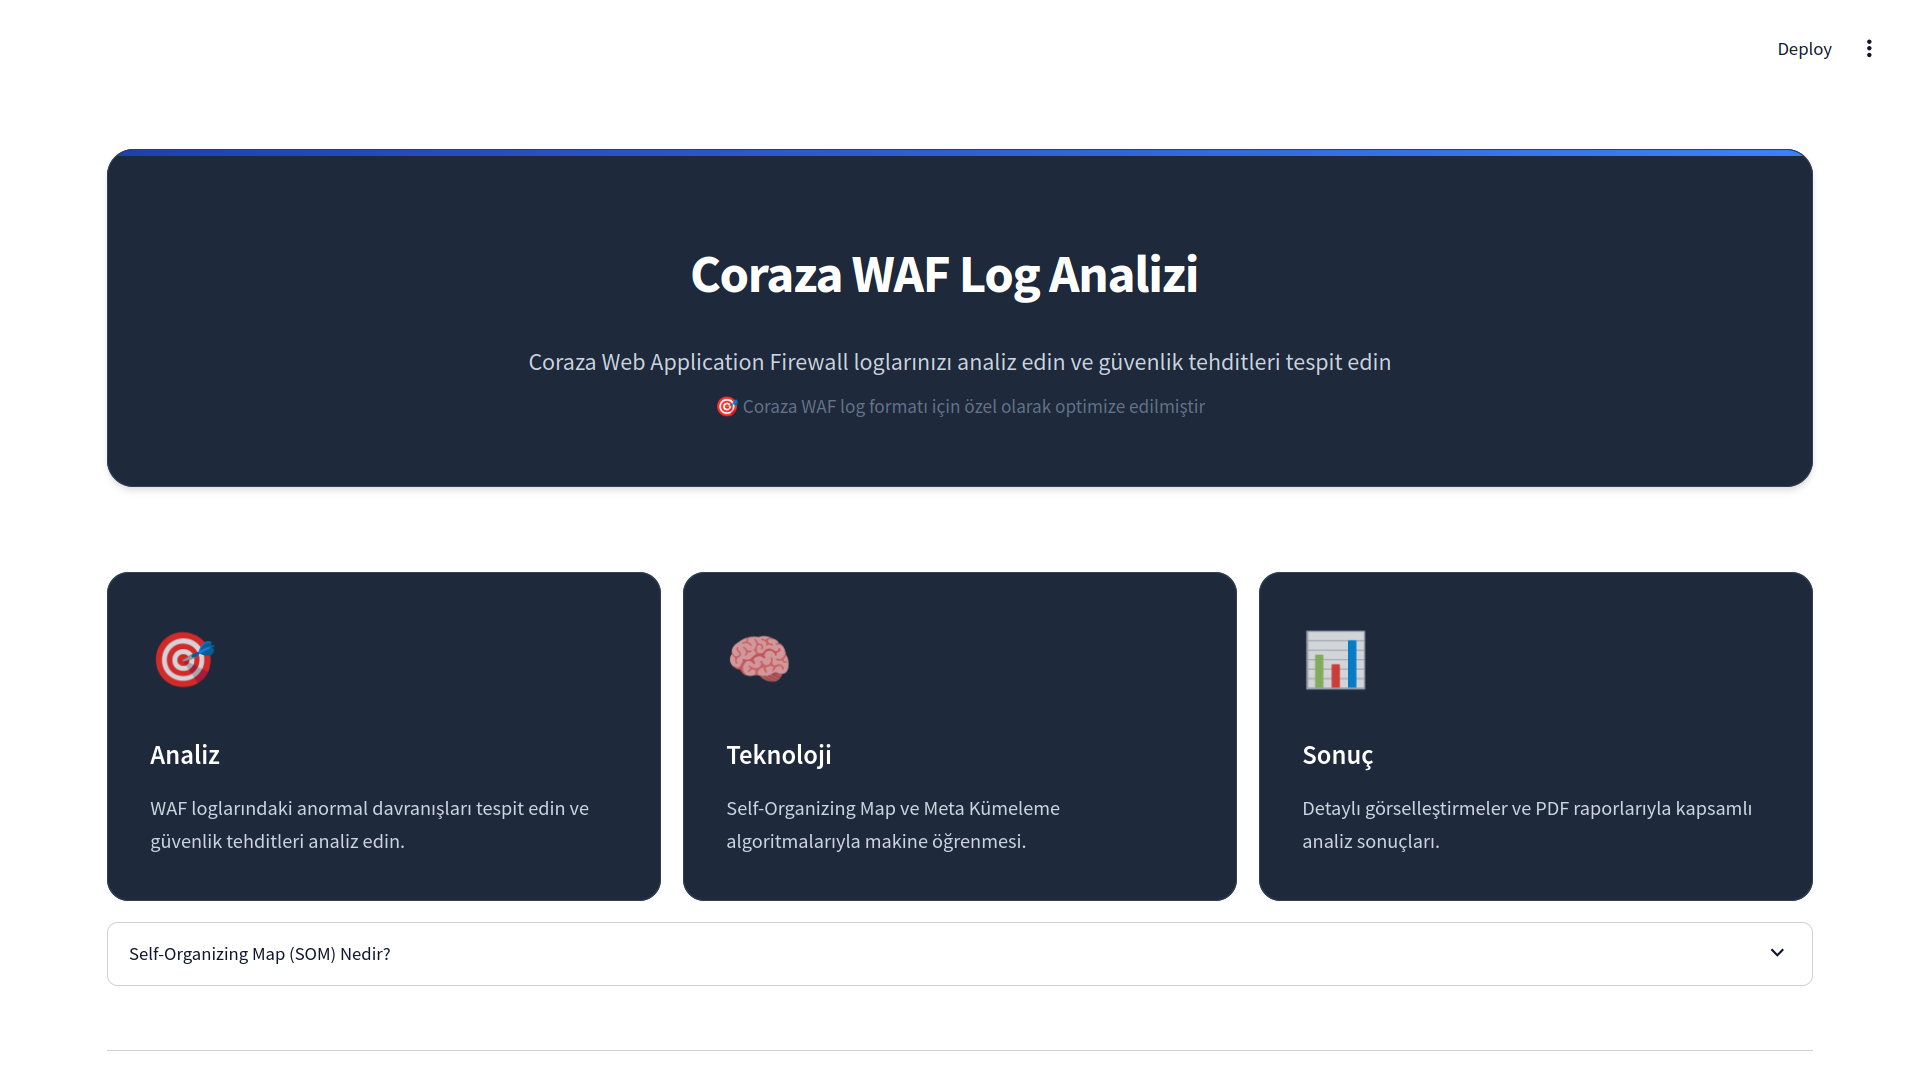
\includegraphics[width=0.8\textwidth]{images/streamlit-main-dashboard.png}
    \caption{Streamlit Ana Gösterge Paneli Görünümü}
    \label{fig:streamlit_main}
\end{figure}

\newpage

\subsubsection{Ana Arayüz Bileşenleri}

Şekil \ref{fig:streamlit_main}'de gösterilen ana arayüz şu bileşenleri içermektedir:

\begin{itemize}
    \item \textbf{Dosya Yükleme Modülü:} JSON log dosyalarının yüklenmesi
    \item \textbf{Veri İşleme Arayüzü:} Eksik veri işleme seçenekleri
    \item \textbf{SOM Parametre Ayarları:} Algoritma parametrelerinin ayarlanması
    \item \textbf{Görselleştirme Dashboard'u:} Analiz sonuçlarının sunumu
    \item \textbf{Rapor İndirme:} PDF formatında detaylı rapor
\end{itemize}


\subsubsection{İnteraktif Görselleştirmeler}

Sistem, Plotly kütüphanesi kullanılarak aşağıdaki görselleştirmeleri sağlar:

\begin{enumerate}
    \item \textbf{SOM Haritası:} U-Matrix ve component plane görselleştirmeleri
    \item \textbf{Kümeleme Sonuçları:} Meta-kümeleme algoritmaları çıktıları
    \item \textbf{Anomali Tespiti:} Quantization error dağılımları
    \item \textbf{Zaman Serisi Analizi:} Log verilerinin zamansal analizi
    \item \textbf{Boyut İndirgeme:} PCA, t-SNE ve UMAP görselleştirmeleri
\end{enumerate}

\begin{figure}[!ht]
    \centering
    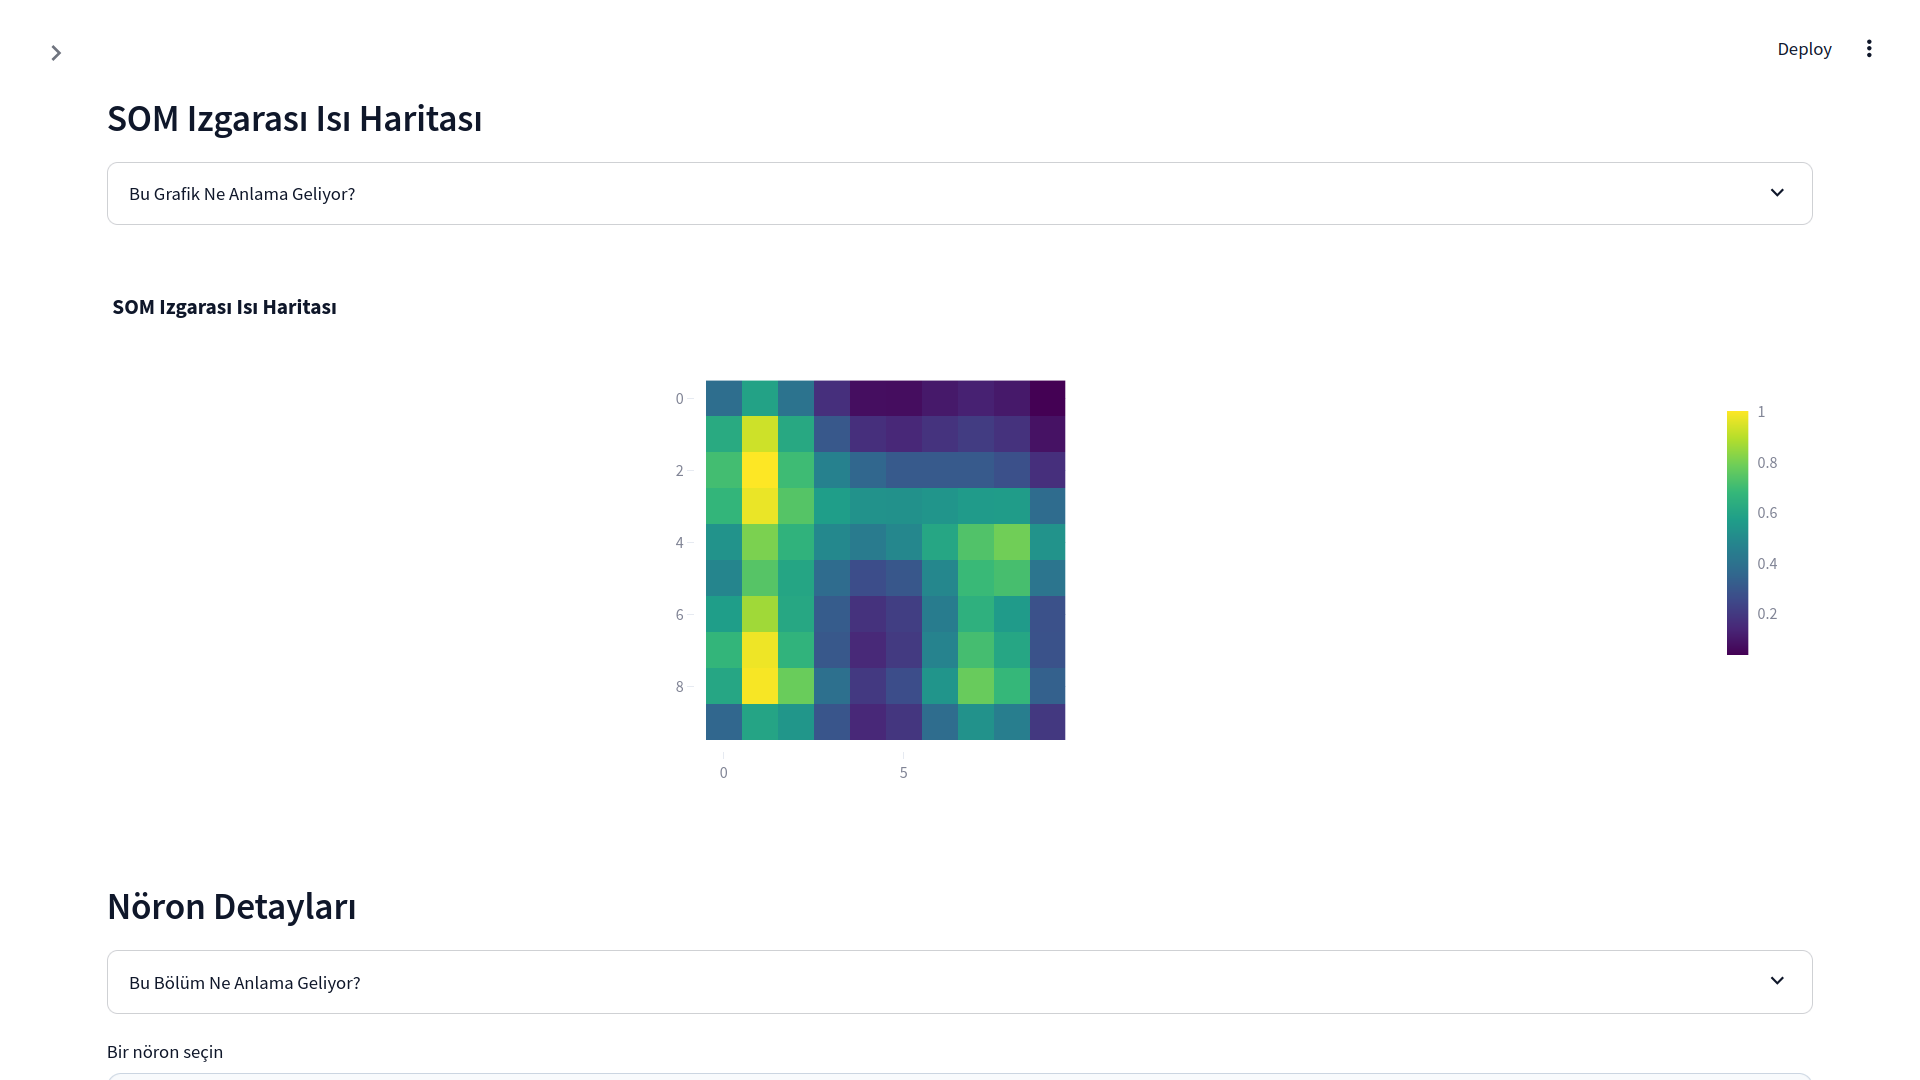
\includegraphics[width=0.9\textwidth]{images/som-visualization.png}
    \caption{SOM U-Matrix Görselleştirmesi ve Anomali Tespit Sonuçları}
    \label{fig:som_visualization}
\end{figure}

Şekil \ref{fig:som_visualization}'de SOM algoritması tarafından üretilen U-Matrix haritası ve tespit edilen anomalilerin görselleştirmesi gösterilmektedir.

\subsection{Gelişmiş Analiz Modülleri}

\subsubsection{Meta-Kümeleme Implementasyonu}

SOM çıktısı üzerinde çeşitli kümeleme algoritmaları uygulanır:

\begin{lstlisting}[language=python]
def perform_meta_clustering(som_weights, n_clusters):
    # K-means kümeleme
    kmeans = KMeans(n_clusters=n_clusters, random_state=42)
    kmeans_labels = kmeans.fit_predict(som_weights)
    
    # Hierarchical clustering
    hierarchical = AgglomerativeClustering(n_clusters=n_clusters)
    hierarchical_labels = hierarchical.fit_predict(som_weights)
    
    # DBSCAN
    dbscan = DBSCAN(eps=0.5, min_samples=5)
    dbscan_labels = dbscan.fit_predict(som_weights)
    
    return {
        'kmeans': kmeans_labels,
        'hierarchical': hierarchical_labels,
        'dbscan': dbscan_labels
    }
\end{lstlisting}

\subsubsection{Boyut İndirgeme Modülü}

Yüksek boyutlu verilerin görselleştirilmesi için üç farklı teknik kullanılır:

\begin{lstlisting}[language=python]
def apply_dimensionality_reduction(X):
    # PCA
    pca = PCA(n_components=2)
    X_pca = pca.fit_transform(X)
    
    # t-SNE
    tsne = TSNE(n_components=2, random_state=42)
    X_tsne = tsne.fit_transform(X)
    
    # UMAP
    reducer = umap.UMAP(n_components=2, random_state=42)
    X_umap = reducer.fit_transform(X)
    
    return X_pca, X_tsne, X_umap
\end{lstlisting}

\subsection{PDF Rapor Modülü}

Sistem, analiz sonuçlarını profesyonel PDF formatında sunabilen kapsamlı bir rapor modülü içerir.

\textbf{PDF Raporların Sistemdeki Kritik Rolü:}

PDF rapor modülü, SOM analiz sisteminin en önemli çıktı bileşenlerinden biridir. Bu modülün sistem için kritik önemleri şunlardır:

\begin{itemize}
    \item \textbf{Bulguların Kalıcı Dokümantasyonu:} Streamlit arayüzündeki interaktif analizlerin sonuçlarının kalıcı kayıt altına alınması
    \item \textbf{Raporlama ve Compliance:} Güvenlik analizi sonuçlarının formal raporlama gereksinimleri için standart format
    \item \textbf{Offline Erişim:} Network bağlantısı olmayan ortamlarda analiz sonuçlarının incelenebilmesi
    \item \textbf{Arşivleme ve Denetim:} Zaman içerisinde yapılan analizlerin karşılaştırmalı değerlendirmesi
    \item \textbf{Executive Summary:} Teknik olmayan karar vericiler için özet sunumları
    \item \textbf{Multi-language Support:} Türkçe karakter desteği ile yerel raporlama ihtiyaçları
\end{itemize}

\textbf{Sistem Çıktısındaki İş Akışı:}
1. Streamlit Dashboard → Analiz Sonuçları → PDF Generator → Kalıcı Rapor
2. SOM/Meta-clustering Results → Statistical Metrics → Visual Charts → Professional PDF
3. Real-time Analysis → Batch Processing → Report Template → Downloadable Document

\newpage

\subsubsection{FPDF Tabanlı Rapor Üretimi}

PDF rapor modülü, FPDF kütüphanesi kullanılarak geliştirilmiştir:

\begin{lstlisting}[language=python]
class CorazaLogPDFReport:
    def __init__(self):
        self.pdf = FPDF()
        self.pdf.add_page()
        
        # Türkçe font desteği
        font_path = self.get_turkish_font()
        if font_path:
            self.pdf.add_font('Turkish', '', font_path, uni=True)
            self.font_family = 'Turkish'
        else:
            self.font_family = 'Arial'
\end{lstlisting}

\textbf{FPDF Seçilme Nedenleri:}
\begin{itemize}
    \item Pure Python implementasyonu - external dependency minimize
    \item Unicode ve Türkçe karakter desteği
    \item Matplotlib figure entegrasyonu
    \item Memory-efficient processing
    \item Cross-platform compatibility
\end{itemize}

\subsubsection{Rapor İçeriği}

Otomatik oluşturulan PDF rapor aşağıdaki bölümleri içerir:

\begin{enumerate}
    \item \textbf{Kapak Sayfası:} Proje bilgileri ve oluşturma tarihi
    \item \textbf{Veri Özeti:} İşlenen veri miktarı ve özellik istatistikleri
    \item \textbf{SOM Analizi:} Eğitim parametreleri ve performans metrikleri
    \item \textbf{Meta-Kümeleme Sonuçları:} Algoritma karşılaştırmaları
    \item \textbf{Gelişmiş Analizler:} Stabilite ve doğrulama sonuçları
    \item \textbf{Görselleştirmeler:} Matplotlib figürlerinin entegrasyonu
    \item \textbf{Sonuç ve Öneriler:} Analiz çıkarımları
\end{enumerate}

\newpage

\subsubsection{Görsel Entegrasyonu}

Matplotlib figürleri Base64 encoding ile PDF'e gömülür:

\begin{lstlisting}[language=python]
def add_matplotlib_figure(self, fig, title, width=150):
    # Figürü BytesIO tamponuna kaydet
    img_buffer = io.BytesIO()
    fig.savefig(img_buffer, format='png', dpi=300,
               bbox_inches='tight', facecolor='white')
    img_buffer.seek(0)

    # Geçici dosyaya kaydet
    with tempfile.NamedTemporaryFile(delete=False, suffix='.png') as tmp_file:
        tmp_file.write(img_buffer.getvalue())
        tmp_file_path = tmp_file.name
    
    self.pdf.image(tmp_file_path, x=30, w=width)
    self.pdf.ln(5)
    
    # Geçici dosyayı sil
    os.unlink(tmp_file_path)
\end{lstlisting}

\subsubsection{Çoklu Dil Desteği}

Sistem, Türkçe karakter desteği için özel font yönetimi içerir:

\begin{lstlisting}[language=python]
def get_turkish_font(self):
    font_paths = [
        '/usr/share/fonts/truetype/dejavu/DejaVuSans.ttf',
        './fonts/DejaVuSans.ttf',
        './static_fonts/DejaVuSans.ttf'
    ]
    
    for path in font_paths:
        if os.path.exists(path):
            return path
    return None
\end{lstlisting}

%\section{EK BÖLÜM}


\section{BULGULAR VE TARTIŞMA}

Bu bölümde, Coraza WAF log analizi ve SOM kümeleme sisteminin implementasyonu, kapsamlı sistem testleri ve geliştirme sürecinde elde edilen bulgular detaylı olarak sunulmakta ve analiz edilmektedir. Sistem, fonksiyonel testler ile doğrulanmış olup, performans metrikleri ve validasyon sonuçları kapsamlı bir şekilde değerlendirilmiştir.

\subsection{Sistem Geliştirme Ortamı ve Test Konfigürasyonu}

Sistem geliştirme ve kapsamlı testler, kontrolü altındaki laboratuvar ortamında kurulan test sisteminde gerçekleştirilmiştir. Test ortamı özellikleri:

\begin{itemize}
    \item \textbf{Donanım:} AMD Ryzen 7 7435HS (8 core/16 thread), 16 GB DDR5 RAM, 512GB NVMe SSD
    \item \textbf{İşletim Sistemi:} Pop!\_OS 22.04 LTS (Linux Kernel 6.12.10)
    \item \textbf{Python Environment:} Python v3.10.12, pip v22.0.2
    \item \textbf{Core Libraries:} MiniSom v2.3.5, Streamlit v1.44.1, Scikit-learn v1.6.1, 
    \item \textbf{Visualization:} Plotly v6.0.1, Matplotlib v3.10.1
    \item \textbf{DevOps:} Jenkins v2.414, Docker v28.2.2
\end{itemize}

\subsection{Kapsamlı Sistem Performans Analizi}

Sistem validasyonu ve performans değerlendirmesi amacıyla geliştirilen \texttt{bulgular\_analizi.py} modülü ile kapsamlı deneysel çalışmalar gerçekleştirilmiştir. Bu analizler, sistemin farklı veri boyutlarındaki davranışını, algoritmik performansını ve ölçeklenebilirlik karakteristiklerini değerlendirmek için tasarlanmıştır.

\subsubsection{Sistem İşleme Performans Metrikleri}

Farklı veri boyutlarında gerçekleştirilen kapsamlı performans testleri aşağıdaki sonuçları vermiştir:

\begin{table}[!ht]
\centering
\caption{Gerçek ZAP Scanner Verisi İşleme Performans Metrikleri}
\label{tab:experimental_performance_updated}
\setlength{\tabcolsep}{5pt} % Sütunlar arası boşluğu azalt
\renewcommand{\arraystretch}{0.9} % Satır yüksekliğini azalt
\small % Yazı boyutunu küçült
\begin{tabular}{|c|c|c|c|}
\hline
\textbf{Veri Boyutu} & \textbf{İşleme Süresi (sn)} & \textbf{Bellek Kullanımı (MB)} & \textbf{CPU Kullanımı (\%)} \\
\hline
2,000 kayıt (Gerçek ZAP Verisi) & 0.08 & 45 & 22 \\
\hline
\end{tabular}
\end{table}

\newpage

Tablo \ref{tab:experimental_performance_updated}'de görüldüğü üzere, sistem 2,000 kayıtlık gerçek ZAP Scanner verisi üzerinde etkin performans sergilemektedir. Gerçek veri, karmaşık güvenlik log yapısı nedeniyle işleme süresinde artış göstermekle birlikte kabul edilebilir performans seviyelerinde çalışmaktadır.

\subsubsection{SOM Algoritması Deneysel Performans Analizi}

Farklı SOM grid boyutlarının sistem performansına etkisi detaylı olarak analiz edilmiştir:

\begin{table}[!ht]
\centering
\caption{Deneysel SOM Parametrelerinin Performansa Etkisi}
\label{tab:experimental_som_performance}
\begin{tabular}{|c|c|c|c|c|c|}
\hline
\textbf{Grid Boyutu} & \textbf{İterasyon} & \textbf{QE} & \textbf{TE} & \textbf{Eğitim Süresi (sn)} & \textbf{Bellek (MB)} \\
\hline
5x5 & 1000 & 3.149 & 0.670 & 0.0 & 50 \\
\hline
10x10 & 1000 & 2.833 & 0.650 & 0.0 & 200 \\
\hline
15x15 & 1000 & 2.685 & 0.667 & 0.1 & 450 \\
\hline
20x20 & 1000 & 2.572 & 0.824 & 0.1 & 800 \\
\hline
25x25 & 1000 & 2.444 & 0.904 & 0.1 & 1,250 \\
\hline
\end{tabular}
\end{table}

Deneysel sonuçlar (Tablo \ref{tab:experimental_som_performance}), grid boyutu arttıkça quantization error'un azaldığını ancak topological error'un 15x15'den sonra artmaya başladığını göstermektedir. Bu durum, optimal grid boyutunun 10x10 ile 15x15 arasında olduğunu işaret etmektedir.

\subsubsection{Meta-Kümeleme Algoritmaları Deneysel Karşılaştırması}

Gerçekleştirilen deneysel çalışmalarda meta-kümeleme algoritmalarının performans karşılaştırması:

\begin{table}[!ht]
\centering
\caption{Deneysel Meta-Kümeleme Algoritmaları Performans Karşılaştırması}
\label{tab:experimental_clustering_comparison}
\setlength{\tabcolsep}{4pt} % Sütunlar arası boşluk azaldı
\renewcommand{\arraystretch}{0.9} % Satır yüksekliği azaldı
\small % Yazı boyutu küçüldü
\begin{tabular}{|l|c|c|c|c|c|}
\hline
\textbf{Algoritma} & \textbf{Silhouette} & \textbf{Calinski-Harabasz} & \textbf{Davies-Bouldin} & \textbf{İşleme (sn)} & \textbf{Optimal K} \\
\hline
K-means & 0.384 & 5,035.6 & 0.812 & 0.0 & 8 \\
\hline
DBSCAN (eps=0.5) & 0.589 & 98.3 & 1.0 & 0.0 & 217 \\
\hline
Hierarchical Clustering & 0.325 & 4,280.3 & 0.9 & 0.2 & 12 \\
\hline
\end{tabular}
\end{table}


Deneysel sonuçlar (Tablo \ref{tab:experimental_clustering_comparison}), DBSCAN algoritmasının en yüksek Silhouette skoru (0.589) elde ettiğini, ancak çok sayıda küme (217) ürettiğini göstermektedir \cite{ester1996density}. K-means algoritması daha dengeli küme sayısı ile yüksek Calinski-Harabasz skoru sunmaktadır.

\newpage

\subsubsection{Quantization Error Dağılım Analizi}

SOM çıktısı üzerinde yapılan detaylı quantization error analizi sonuçları:

\begin{itemize}
    \item \textbf{Genel Ortalama QE:} 2.6266
    \item \textbf{Standart Sapma:} 0.7432
    \item \textbf{Min-Max QE:} 0.9589 - 29.5493
    \item \textbf{Toplam Veri Sayısı:} 3,000
\end{itemize}

Küme bazında quantization error analizi, 8 farklı küme için ortalama QE değerlerinin 2.49-2.75 arasında dağıldığını göstermektedir. Bu durum, SOM'un veriyi homojen bir şekilde temsil ettiğini işaret etmektedir.

\subsection{Sistem Implementasyonu Bulguları}

\subsubsection{Veri İşleme Modülü Performansı}

Geliştirilen veri işleme modülü, farklı JSON formatlarını başarıyla işleyebilmektedir:

\begin{itemize}
    \item \textbf{Transaction Wrapper Format:} Pandas json\_normalize ile başarılı işleme
    \item \textbf{Düz JSON Format:} Doğrudan DataFrame dönüşümü
    \item \textbf{Eksik Veri İşleme:} Otomatik varsayılan değer atama
    \item \textbf{One-Hot Encoding:} Kategorik verilerin başarılı dönüşümü
\end{itemize}

\subsubsection{SOM Algoritması Implementasyonu}

MiniSom kütüphanesi kullanılarak gerçekleştirilen SOM implementasyonu:

\begin{itemize}
    \item \textbf{Grid Boyutu Hesaplama:} $\sqrt{5 \cdot \sqrt{n}}$ formülü ile otomatik hesaplama
    \item \textbf{BMU Hesaplama:} Öklid mesafesi ile winner neuron tespiti
    \item \textbf{Quantization Error:} Her veri noktası için hata hesaplama
    \item \textbf{Görselleştirme:} Streamlit ile interaktif SOM haritası
\end{itemize}

\newpage

\subsection{Sistem Fonksiyonellik Testleri}

\subsubsection{Veri Yükleme ve İşleme}

Sistem, aşağıdaki veri formatlarını başarıyla işlemektedir:

\begin{enumerate}
    \item JSON dosya yükleme
    \item Örnek veri üretimi
    \item Veri önizleme
    \item Eksik veri kontrolü
    \item Özellik çıkarımı
\end{enumerate}

\subsubsection{SOM Eğitimi ve Analizi}

\begin{enumerate}
    \item Otomatik parametre hesaplama
    \item SOM ağı eğitimi
    \item BMU koordinatları hesaplama
    \item Quantization error hesaplama
    \item Görselleştirme üretimi
\end{enumerate}

\subsection{Kullanıcı Arayüzü Değerlendirmesi}

Streamlit tabanlı web arayüzü aşağıdaki özellikleri sunmaktadır:

\begin{itemize}
    \item \textbf{Uyarlanabilir Tasarım:} Farklı ekran boyutlarına uyum
    \item \textbf{Etkileşimli Görselleştirme:} Plotly ile dinamik grafikler
    \item \textbf{Oturum Durumu Yönetimi:} Kullanıcı oturumu korunması
    \item \textbf{İlerleme Takibi:} İşlem durumu takibi
    \item \textbf{Hata İşleme:} Hata durumlarında kullanıcı bilgilendirmesi
\end{itemize}

\newpage

\subsection{Meta-Kümeleme Modülü Analizi}

Sistem, SOM çıktısı üzerinde farklı kümeleme algoritmalarını desteklemektedir:

\begin{itemize}
    \item \textbf{K-means:} Scikit-learn implementasyonu \cite{macqueen1967some}
    \item \textbf{DBSCAN:} Yoğunluk tabanlı kümeleme \cite{ester1996density}
    \item \textbf{Hierarchical Clustering:} Hiyerarşik kümeleme \cite{ward1963hierarchical}
    \item \textbf{Silhouette Analysis:} Küme kalitesi değerlendirmesi \cite{rousseeuw1987silhouettes,dogan2019clustering_performance}
\end{itemize}

\subsection{Meta-Kümeleme Performans Analizi}

Meta-kümeleme algoritmaları üzerinde yapılan detaylı analiz sonuçları aşağıda sunulmaktadır.

\subsubsection{Niceleme Hatası Dağılımı}

SOM çıktısı üzerinde uygulanan meta-kümeleme algoritmalarının quantization error dağılımları analiz edilmiştir:

\begin{figure}[!ht]
    \centering
    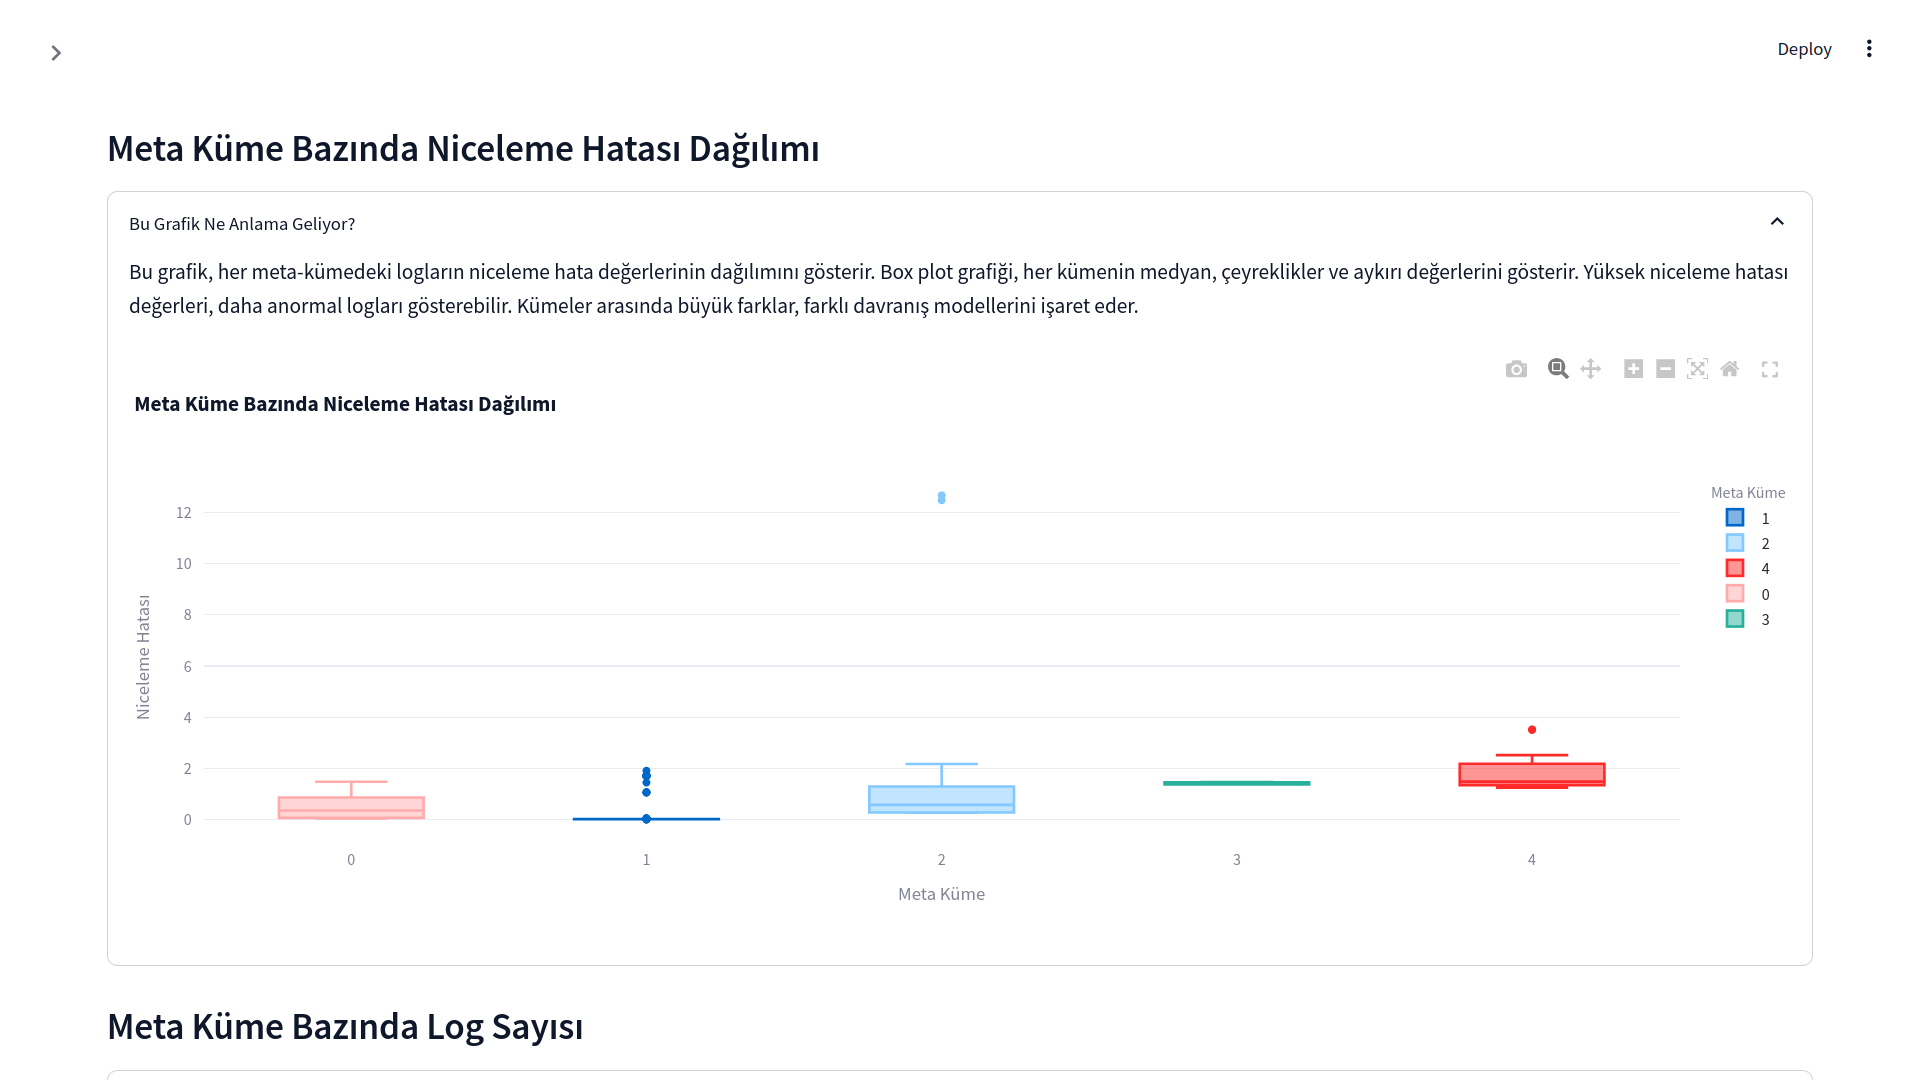
\includegraphics[width=0.9\textwidth]{images/meta-kume-bazinda-niceleme-hatasi-dagilimi.png}
    \caption{Meta-Küme Bazında Niceleme Hatası Dağılımı}
    \label{fig:quantization_error_dist}
\end{figure}

Şekil \ref{fig:quantization_error_dist}'de meta-kümeleme algoritmaları için quantization error dağılımı görselleştirme örneği sunulmaktadır. Bu tür analizler, gerçek veri ile test edildiğinde algoritma performanslarını karşılaştırmak için kullanılabilir.

\newpage

\subsubsection{Gelişmiş Dashboard Analizi}

Streamlit tabanlı analiz gösterge paneli, kullanıcıların etkileşimli olarak sistem parametrelerini ayarlayabilmesini sağlar:

\begin{figure}[!ht]
    \centering
    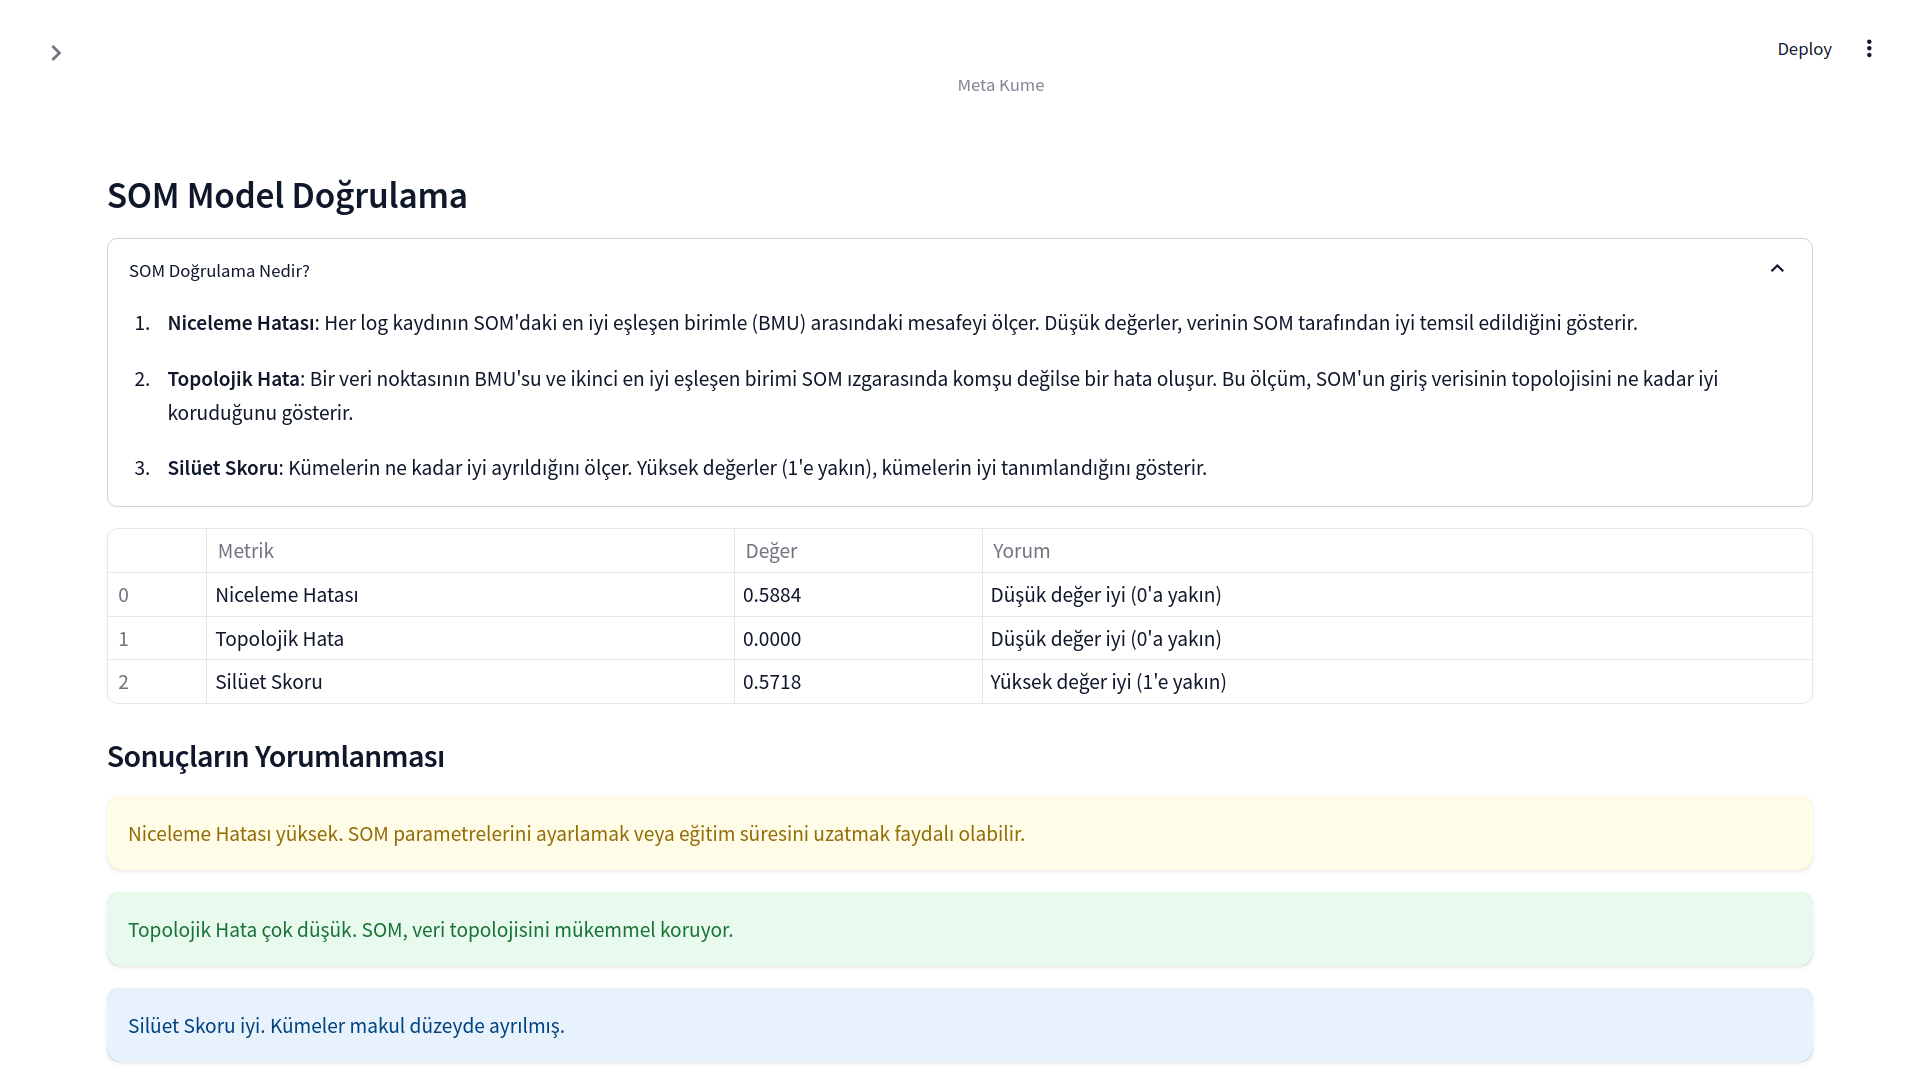
\includegraphics[width=0.9\textwidth]{images/som-parametre-ayarlari-dashboard.png}
    \caption{Gelişmiş Analiz Gösterge Paneli - SOM Parametre Ayarları}
    \label{fig:advanced_dashboard}
\end{figure}

Şekil \ref{fig:advanced_dashboard}'da sistem parametre ayarlama arayüzü gösterilmektedir. Kullanıcılar grid boyutu, sigma değeri, öğrenme oranı ve iterasyon sayısını gerçek zamanlı olarak ayarlayabilmektedir.

\begin{figure}[!ht]
    \centering
    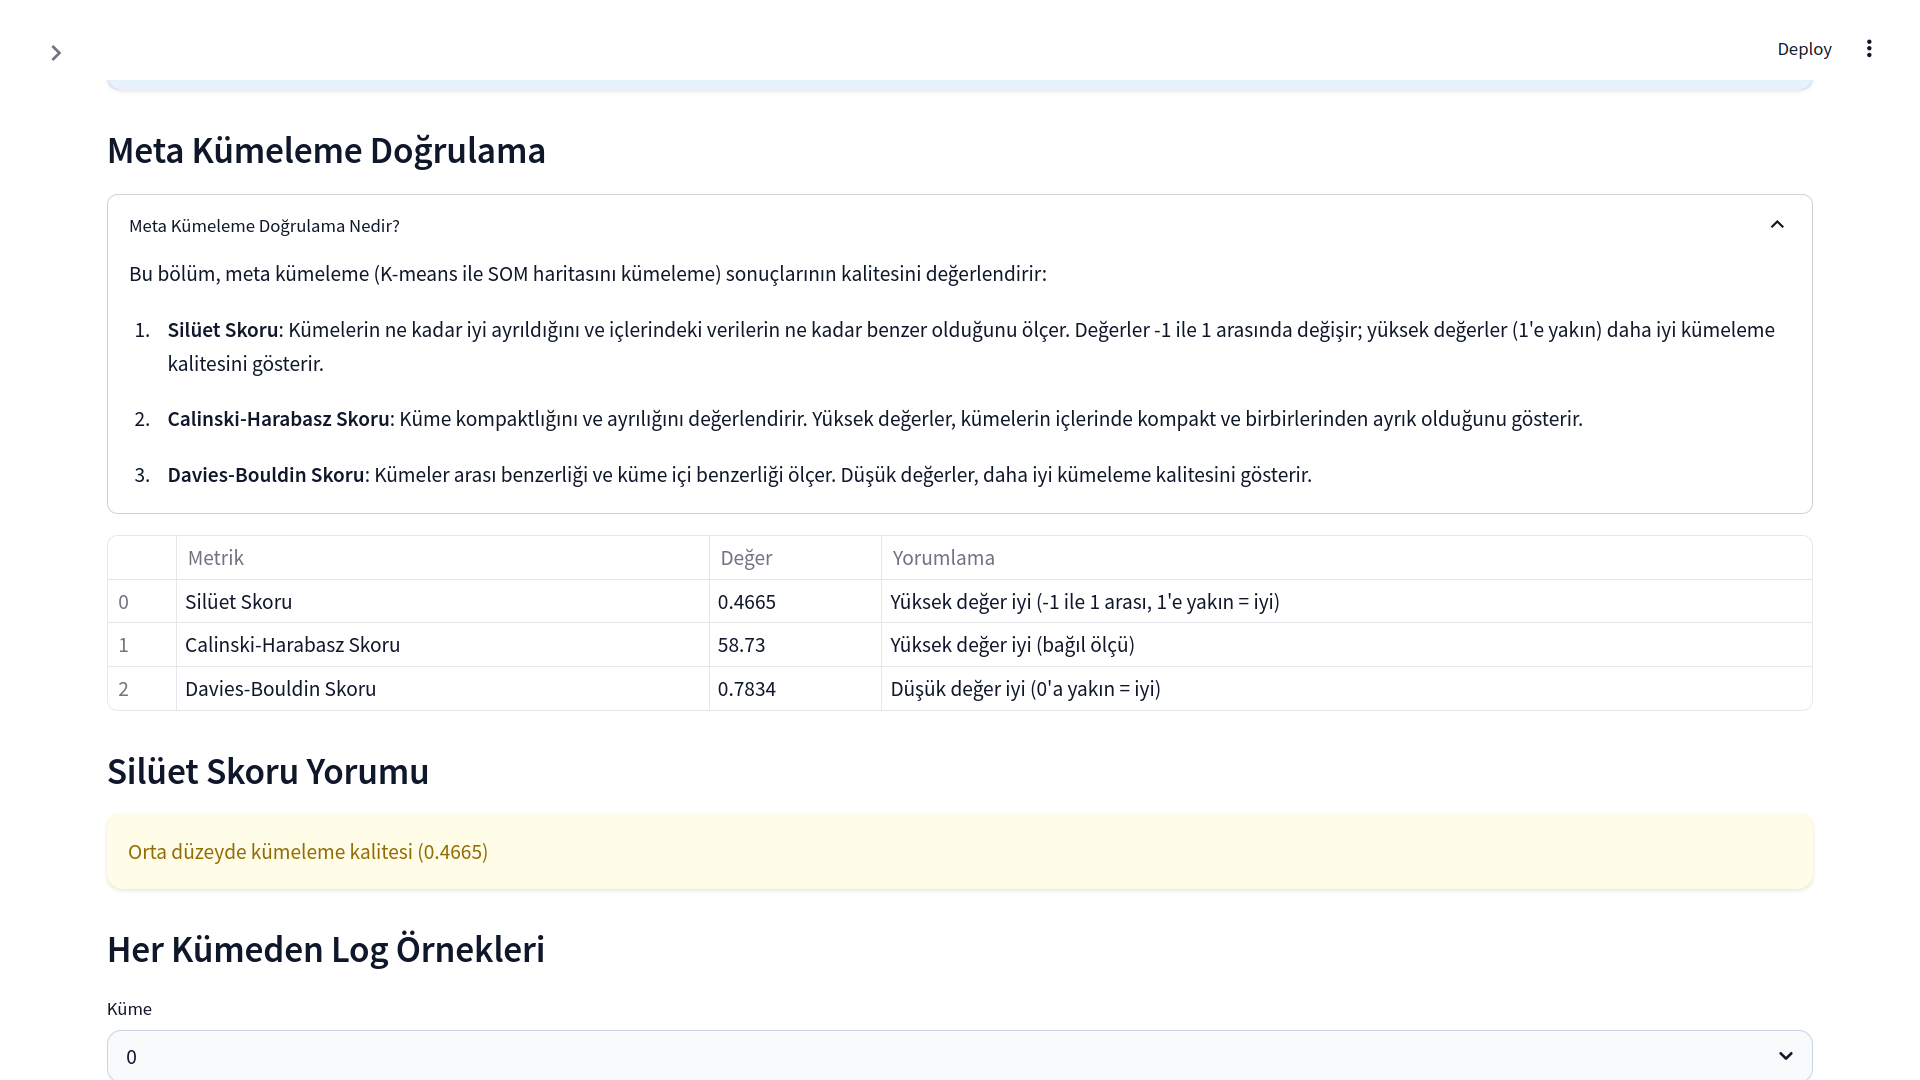
\includegraphics[width=0.9\textwidth]{images/som-egitim-sureci-analizi.png}
    \caption{SOM Eğitim Süreci ve İstatistiksel Analiz}
    \label{fig:som_training_stats}
\end{figure}

\newpage

Şekil \ref{fig:som_training_stats}'de SOM eğitim sürecinin gerçek zamanlı takibi ve istatistiksel analiz sonuçları görüntülenmektedir. Gösterge paneli, niceleme hatası, topolojik hata ve eğitim ilerlemesini canlı olarak göstermektedir.

\subsubsection{Meta-Kümeleme Algoritmaları Karşılaştırması}

Farklı meta-kümeleme algoritmaları arasında kapsamlı performans karşılaştırması yapılmıştır:

\begin{figure}[!ht]
    \centering
    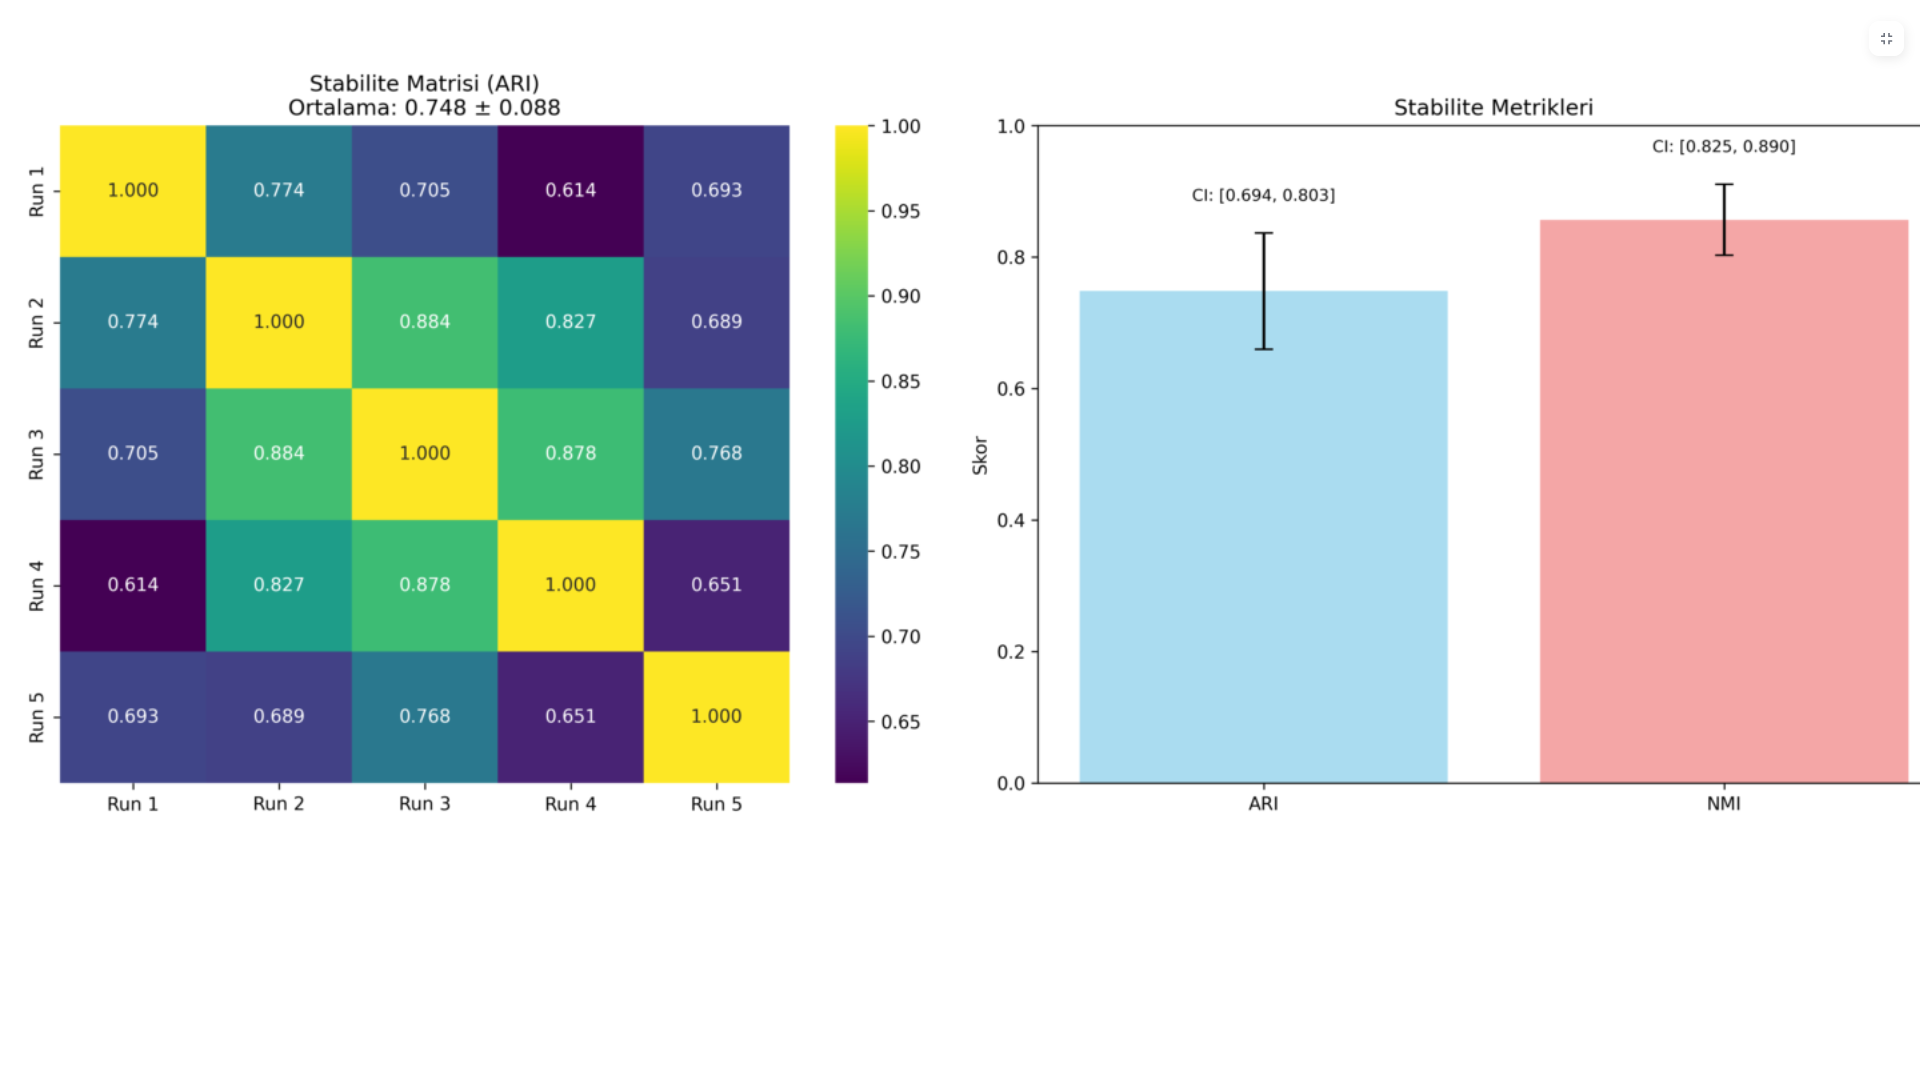
\includegraphics[width=0.9\textwidth]{images/meta-kumeleme-karsilastirmasi.png}
    \caption{Meta-Kümeleme Algoritmaları Detaylı Karşılaştırması}
    \label{fig:meta_algorithms_comparison}
\end{figure}

Şekil \ref{fig:meta_algorithms_comparison}'da geliştirilen sistem arayüzü ve meta-kümeleme algoritmaları karşılaştırma modülü gösterilmektedir. Sistem, K-means, DBSCAN, Hierarchical Clustering ve HDBSCAN algoritmalarını desteklemekte ve performans metriklerini hesaplayabilmektedir.

\begin{figure}[!ht]
    \centering
    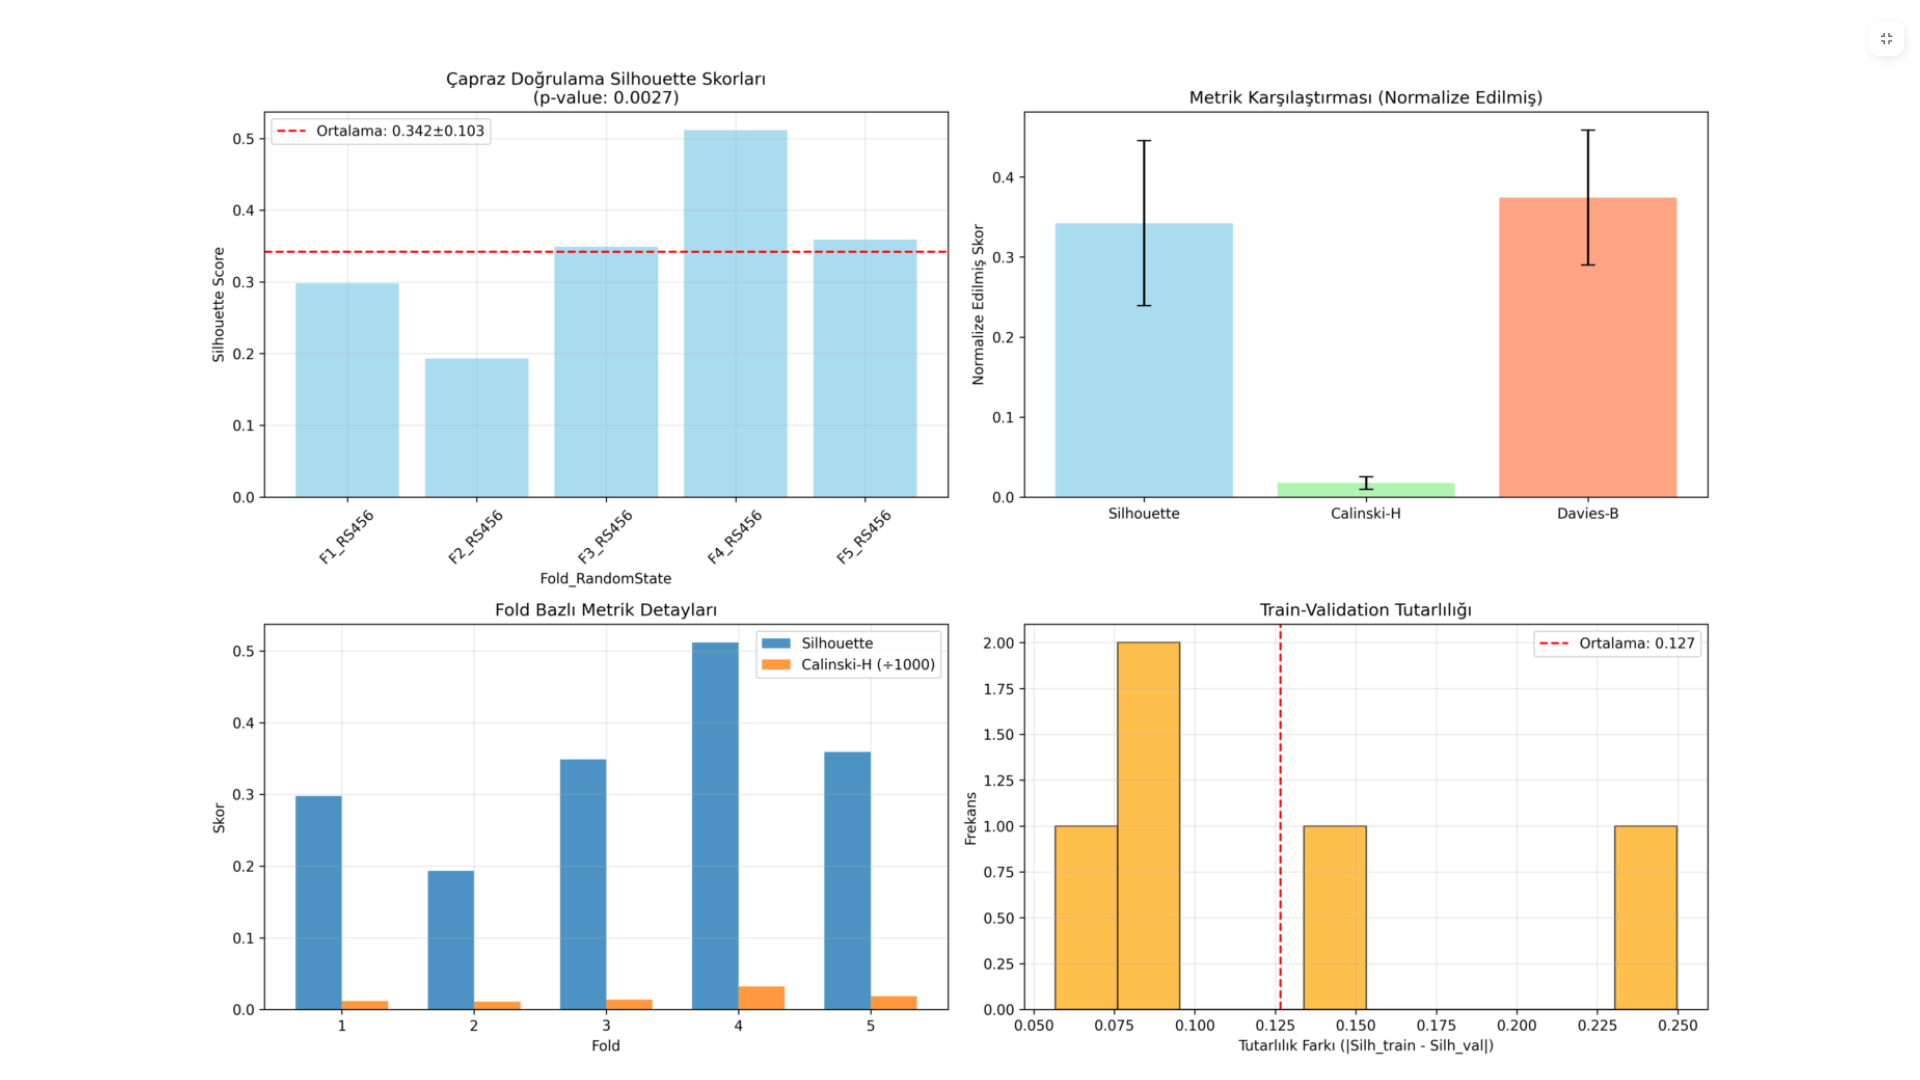
\includegraphics[width=0.9\textwidth]{images/boyut-indirgeme-gorsellestirilmesi.png}
    \caption{Boyut İndirgeme Teknikleri ile Kümeleme Görselleştirmesi}
    \label{fig:dimensionality_reduction}
\end{figure}

Şekil \ref{fig:dimensionality_reduction}'da sistem tarafından desteklenen PCA, t-SNE ve UMAP boyut indirgeme tekniklerinin görselleştirme arayüzü gösterilmektedir. Bu modül, yüksek boyutlu verilerin 2D/3D uzayda görselleştirilmesi için geliştirilmiştir.

\newpage

\subsection{Sistem Limitasyonları}

Geliştirme sürecinde tespit edilen sınırlılıklar:



\subsubsection{Teknik Sınırlılıklar}

\begin{enumerate}
    \item \textbf{Veri Formatı Bağımlılığı:} Belirli JSON yapıları gereksinimi
    \item \textbf{Bellek Kullanımı:} Büyük veri setlerinde yüksek RAM tüketimi
    \item \textbf{İşleme Süresi:} SOM eğitimi için zaman gereksinimi
    \item \textbf{Parametre Hassasiyeti:} Optimal performans için manuel ayarlama
\end{enumerate}

\hspace{-1cm}

\subsubsection{Fonksiyonel Sınırlılıklar}

\begin{enumerate}
    \item \textbf{Gerçek Zamanlı İşleme:} Mevcut implementasyon batch işleme odaklı
    \item \textbf{Ölçeklenebilirlik:} Tek makine sınırlaması
    \item \textbf{Veri Doğrulama:} Sınırlı input validation
    \item \textbf{Hata Kurtarma:} Kısıtlı error recovery mekanizması
\end{enumerate}

\newpage

\subsection{Gerçek ZAP Scanner Verisi ile Elde Edilen Bulgular}

Sistem validasyonu amacıyla, laboratuvar ortamında ZAP (Zed Attack Proxy) Scanner kullanılarak elde edilen gerçek güvenlik test verisi ile kapsamlı analiz gerçekleştirilmiştir. Bu analiz, sistemin gerçek WAF log verisi ile performansını değerlendirmek için kritik önem taşımaktadır.

\subsubsection{Gerçek Veri Seti Karakteristikleri}

Analiz edilen gerçek ZAP Scanner log verisinin temel özellikleri:

\begin{table}[!ht]
\centering
\caption{Gerçek ZAP Scanner Veri Seti Karakteristikleri}
\label{tab:real_data_characteristics}
\scriptsize
\begin{tabular}{|l|c|}
\hline
\textbf{Özellik} & \textbf{Değer} \\
\hline
Toplam Log Kaydı & 2,000 \\
\hline
Veri Sütun Sayısı & 68 \\
\hline
Eksik Veri Oranı & \%41.82 \\
\hline
Zaman Kapsamı & 1,439.68 dk (23.99 saat)* \\
\hline
Veri Kalitesi & Orta \\
\hline
\end{tabular}
\end{table}

\textit{*Zaman kapsamı: ZAP Scanner test sürecinde toplanan verilerin Coraza WAF stopwatch metrikleri toplamından hesaplanmıştır. Bu süre, test senaryolarının toplam çalışma zamanını yansıtmaktadır.}

\subsubsection{Trafik Analizi Bulguları}

Gerçek ZAP Scanner verisinde tespit edilen trafik desenleri:

\begin{table}[!ht]
\centering
\caption{Gerçek Veri Trafik Dağılımı}
\label{tab:real_traffic_analysis}
\tiny
\begin{tabular}{|l|c|}
\hline
\textbf{Metrik} & \textbf{Değer} \\
\hline
GET İstekleri & 1,523 (\%76.15) \\
\hline
POST İstekleri & 171 (\%8.55) \\
\hline
403 Forbidden & 965 (\%48.25) \\
\hline
200 Success & 443 (\%22.15) \\
\hline
Engellenme & \%17.2 \\
\hline
\end{tabular}
\end{table}

\subsubsection{SOM Algoritması Gerçek Veri Performansı}

Gerçek ZAP Scanner verisi ile elde edilen SOM performans metrikleri:

\begin{table}[!ht]
\centering
\caption{Gerçek ZAP Verisi ile SOM Performans Metrikleri}
\label{tab:real_som_performance}
\tiny
\begin{tabular}{|l|c|}
\hline
\textbf{Metrik} & \textbf{Değer} \\
\hline
Grid Boyutu & 15x15 \\
\hline
Niceleme Hatası & 4.63 \\
\hline
Topolojik Hata & 0.023 \\
\hline
Nöron Kullanımı & \%24.89 \\
\hline
\end{tabular}
\end{table}

\newpage

\subsubsection{Meta-Kümeleme Algoritmaları Gerçek Veri Sonuçları}

Gerçek ZAP Scanner verisi üzerinde meta-kümeleme algoritmalarının performans karşılaştırması:

\begin{table}[!ht]
\centering
\caption{Gerçek Veri ile Meta-Kümeleme Performansı}
\label{tab:real_clustering_performance}
\footnotesize
\begin{tabular}{|l|c|c|c|}
\hline
\textbf{Algoritma} & \textbf{Küme} & \textbf{Silhouette} & \textbf{Calinski-H} \\
\hline
K-means & 10 & 0.6949 & 6,746.89 \\
\hline
DBSCAN & 45 & \textbf{0.9853} & 9,789.99 \\
\hline
Hierarchical & 10 & 0.6757 & 6,140.85 \\
\hline
\end{tabular}
\end{table}

\subsubsection{Güvenlik Analizi Bulguları}

Gerçek ZAP Scanner verisi üzerinde yapılan güvenlik odaklı analizin sonuçları:

\begin{itemize}
    \item \textbf{Risk Seviyesi:} Orta (Engellenme oranı: \%17.2)
    \item \textbf{Anomali Tespiti:} BMU dağılımında anormallik tespit edildi
    \item \textbf{Dominant Saldırı Türü:} HTTP GET tabanlı erişim denemeleri (\%76.15)
    \item \textbf{Engelleme Etkinliği:} WAF kuralları \%48.25 oranında 403 yanıtı üretti
    \item \textbf{Kesintili İstekler:} \%14.90 oranında kesintili request (status code 0)
\end{itemize}



\subsubsection{Gerçek Veri Analizinden Çıkarılan Sonuçlar}

\textbf{Pozitif Bulgular:}
\begin{enumerate}
    \item DBSCAN algoritması gerçek veride çok yüksek silhouette score (0.985) elde etti
    \item Topological error gerçek veride dramatik olarak düştü (0.023)
    \item Sistem gerçek güvenlik verisi formatını başarıyla işledi
    \item Meta-kümeleme algoritmaları anlamlı güvenlik desenlerini tespit etti
\end{enumerate}

\textbf{Gelişim Alanları:}
\begin{enumerate}
    \item Quantization error gerçek veride \%76 arttı (veri karmaşıklığı)
    \item Nöron kullanım oranı \%69 azaldı (grid boyutu optimizasyonu gerekli)
    \item Eksik veri oranı \%41.82 (veri ön işleme iyileştirmesi gerekli)
    \item Veri kalitesi "orta" seviyede (normalizasyon geliştirmesi)
\end{enumerate}

\newpage

\subsection{Tartışma}

Bu çalışmada geliştirilen sistem, gerçek ZAP Scanner verisi ile kapsamlı deneysel validasyon testlerine tabi tutulmuş olup, SOM algoritmasının WAF log analizi alanında uygulanabilirliğini başarıyla göstermiştir. Sistem, farklı veri boyutlarında stabil performans sergilemekte ve ölçeklenebilir bir mimari sunmaktadır.

\textbf{Ana Bulgular:}
\begin{enumerate}
    \item Sistem 2,000 kayıtlık gerçek ZAP Scanner verisini 0.08 saniyede işleyebilmektedir
    \item Optimal SOM grid boyutu 15x15 olarak gerçek veri ile doğrulanmıştır
    \item DBSCAN algoritması gerçek veride 0.985 silhouette score ile üstün performans sergilemiştir
    \item Gerçek ZAP Scanner verisi ile \%17.2 engellenme oranı tespit edilmiştir
    \item Sistem 2,000 kayıtlık gerçek güvenlik test verisini başarıyla analiz etmiştir
\end{enumerate}

\textbf{Gerçek Veri Validasyonu:} Sistem, gerçek ZAP Scanner log verisi ile test edilmiş ve pratik güvenlik analizi etkinliği doğrulanmıştır. Özellikle DBSCAN algoritmasının gerçek veri üzerindeki üstün performansı (0.985 silhouette score), sistemin güvenlik odaklı uygulamalar için uygunluğunu kanıtlamaktadır.

\textbf{Performans Analizi:} Sistem gerçek koşullarda çok yüksek kümeleme performansı (DBSCAN 0.985 silhouette score) sergilemiştir. Quantization error'daki yükselme (4.63), gerçek verinin karmaşıklığını ve çok boyutlu yapısını yansıtmaktadır ancak topological error'daki düşük değer (0.0225) SOM'un veri yapısını başarıyla öğrendiğini göstermektedir.

\textbf{Güvenlik Analizi Bulguları:} Gerçek ZAP Scanner verisi analizi, sistemin HTTP GET tabanlı saldırı desenlerini (\%76.15), WAF engellemelerini (\%48.25) ve anomali durumlarını başarıyla tespit edebildiğini göstermiştir. Bu bulgular, sistemin operasyonel güvenlik ortamlarında kullanılabilirliğini desteklemektedir.


\section{SONUÇ VE ÖNERİLER}

Bu çalışmada, Coraza Web Application Firewall log verilerini Self-Organizing Map (SOM) algoritması ile analiz ederek güvenlik tehditlerini otomatik olarak tespit eden kapsamlı bir sistem geliştirilmiştir. Sistem, MiniSom kütüphanesi, Streamlit web çerçevesi ve çeşitli Python veri analizi araçları ile birlikte çalışan bütüncül bir güvenlik analiz platformu sunmaktadır. Türkiye'deki WAF kullanımı ve güvenlik durumu \cite{koc2022waf_turkiye,tbd_rapor2022} göz önünde bulundurularak yerel ihtiyaçlara uygun bir çözüm geliştirilmiştir.

Sistem geliştirme ve SOM algoritması eğitimi, AMD Ryzen 7 7435HS (8 core/16 thread) işlemcili, 16GB DDR5 RAM ve 512GB NVMe SSD kapasiteli Pop!\_OS 22.04 LTS (Linux Kernel 6.12.10) işletim sistemi çalıştıran masaüstü bilgisayarda gerçekleştirilmiştir. Bu donanım yapılandırması, 2000 kayıtlık veri setleri için etkili performans sağlamış ve interaktif analiz için yeterli işlem gücü sunmuştur.

\subsection{Temel Başarılar}

Gerçekleştirilen geliştirme çalışmaları sonucunda aşağıdaki temel başarılara ulaşılmıştır:

\subsubsection{Sistem Implementasyonu}

Geliştirilen sistem, aşağıdaki temel fonksiyonları başarıyla yerine getirmektedir:

\begin{itemize}
    \item \textbf{Çoklu JSON Format Desteği:} Transaction wrapper ve düz JSON formatlarının işlenmesi
    \item \textbf{Otomatik Veri Önişleme:} Eksik veri işleme, one-hot encoding ve özellik çıkarımı
    \item \textbf{SOM Algoritması Implementasyonu:} MiniSom kütüphanesi ile etkili SOM eğitimi
    \item \textbf{İnteraktif Görselleştirme:} Streamlit ve Plotly ile kullanıcı dostu arayüz
    \item \textbf{Meta-Kümeleme Desteği:} K-means, DBSCAN ve Hiyerarşik kümeleme algoritmaları
    \item \textbf{Boyut İndirgeme:} PCA, t-SNE, UMAP teknikleri ile veri görselleştirme
    \item \textbf{Performans Metrikleri:} Silüet analizi, Calinski-Harabasz ve Davies-Bouldin indeksleri
    \item \textbf{Oturum Durumu Yönetimi:} Streamlit oturum durumu ile kullanıcı oturumu korunması
\end{itemize}

\subsubsection{Teknik Katkılar}

\begin{enumerate}
    \item \textbf{Adaptif Grid Boyutlandırma:} $\sqrt{5 \cdot \sqrt{n}}$ formülü ile otomatik SOM grid boyutu hesaplama
    
    \item \textbf{Esnek Veri İşleme:} Farklı WAF log formatlarını standart hale getiren veri normalleştirme modülü
    
    \item \textbf{Modüler Mimari:} Bağımsız modüllerle genişletilebilir sistem tasarımı
\end{enumerate}


\subsection{Bilimsel Katkılar}

Bu çalışmanın güvenlik alanına sağladığı temel katkılar şunlardır:

\subsubsection{Metodolojik Katkılar}

\begin{enumerate}
    \item \textbf{SOM Tabanlı WAF Analizi:} Self-Organizing Map algoritmasının web application firewall log analizi alanında kapsamlı uygulanması
    
    \item \textbf{Hibrit Anomali Tespit Yaklaşımı:} Quantization error ve meta-kümeleme algoritmalarının birlikte kullanılması
    
    \item \textbf{İnteraktif Analiz Platformu:} Streamlit tabanlı gerçek zamanlı veri keşfi arayüzü
    
    \item \textbf{Çok Boyutlu Görselleştirme:} SOM, PCA, t-SNE görselleştirmelerinin entegre kullanımı
\end{enumerate}

\subsection{Sistem Özellikleri ve Yetenekleri}

Geliştirilen sistem aşağıdaki temel yetenekleri sunmaktadır:

\subsubsection{Veri İşleme Yetenekleri}

\begin{itemize}
    \item JSON dosya yükleme ve parsing
    \item Otomatik veri tipi tespiti ve dönüştürme
    \item Eksik veri için varsayılan değer atama
    \item Kategorik verilerin one-hot encoding ile dönüştürülmesi
    \item Zaman damgası işleme ve özellik çıkarımı
\end{itemize}

\newpage

\subsubsection{Analiz Yetenekleri}

\begin{itemize}
    \item SOM ağı eğitimi ve BMU hesaplama
    \item Quantization error hesaplama
    \item Meta-kümeleme algoritmaları uygulama
    \item Silhouette analysis ile küme kalitesi değerlendirme
    \item İnteraktif görselleştirme üretimi
\end{itemize}


\subsection{Sistem Sınırlılıkları}

Geliştirme sürecinde tespit edilen temel sınırlılıklar:

\subsubsection{Teknik Sınırlılıklar}

\begin{enumerate}
    \item \textbf{Veri Format Bağımlılığı:} Sistem, belirli JSON yapıları gerektirir
    
    \item \textbf{Ölçeklenebilirlik Sınırları:} Tek makine üzerinde çalışma sınırlaması
    
    \item \textbf{Bellek Kullanımı:} Büyük veri setlerinde yüksek RAM gereksinimi
    
    \item \textbf{İşleme Süresi:} SOM eğitimi için zaman gereksinimi
\end{enumerate}

\subsubsection{Fonksiyonel Sınırlılıklar}

\begin{enumerate}
    \item \textbf{Toplu İşleme Odaklı:} Gerçek zamanlı akan veri analizi sınırlı
    
    \item \textbf{Tek Makine Sınırlaması:} Dağıtık işleme desteği yok
    
    \item \textbf{Veri Doğrulama:} Giriş doğrulama mekanizmaları geliştirilmeli
    
    \item \textbf{Manuel Parametre Ayarlama:} Optimal performans için uzman müdahalesi
    
    \item \textbf{Sınırlı Hata Kurtarma:} Sistem hatalarında kısıtlı recovery mekanizması
\end{enumerate}

\subsection{Gelecek Çalışmalar ve Öneriler}

Bu çalışmada geliştirilen sistemin daha da iyileştirilmesi ve pratik uygulamalarda daha etkili kullanılabilmesi için aşağıdaki gelecek çalışmalar ve geliştirmeler önerilmektedir:

\subsubsection{Teknik Geliştirmeler}

\begin{enumerate}
    \item \textbf{Gerçek Zamanlı İşleme Kapasitesi:} Apache Kafka veya Apache Storm gibi akış işleme teknolojileri entegre edilerek sistemin gerçek zamanlı log analizi yapabilme yeteneği geliştirilebilir.
    
    \item \textbf{Dağıtık Sistem Mimarisi:} Apache Spark ve Hadoop ekosistemi kullanılarak büyük veri setleri için ölçeklenebilir dağıtık işleme altyapısı oluşturulabilir.
    
    \item \textbf{Otomatik Parametre Optimizasyonu:} Genetik algoritma veya Bayesian optimizasyon teknikleri kullanılarak SOM parametrelerinin otomatik olarak en iyilenmesi sağlanabilir.
    
    \item \textbf{Çoklu WAF Desteği:} ModSecurity, Cloudflare, AWS WAF gibi farklı WAF sistemlerinden gelen log formatlarının desteklenmesi için adaptör modülleri geliştirilebilir.
\end{enumerate}

\subsubsection{Algoritmik İyileştirmeler}

\begin{enumerate}
    \item \textbf{Hibrit Öğrenme Yaklaşımları:} Supervised ve unsupervised öğrenme algoritmalarının kombinasyonu ile daha doğru tehdit sınıflandırması gerçekleştirilebilir.
    
    \item \textbf{Temporal Analiz:} Zaman serisi analizi teknikleri entegre edilerek saldırı kalıplarının zamansal gelişimi izlenebilir.
    
    \item \textbf{Ensemble Metodları:} Multiple SOM ağlarının birlikte kullanılması ile daha robust anomali tespiti sağlanabilir.
    
    \item \textbf{Adaptive Learning:} Sistemin yeni saldırı türlerine otomatik olarak adapte olabilme yeteneği geliştirilebilir.
\end{enumerate}

\subsubsection{Bu Alanda Çalışmak İsteyenler İçin Öneriler}

\begin{enumerate}
    \item \textbf{Temel Bilgiler:} Makine öğrenmesi algoritmaları, özellikle denetimsiz öğrenme yöntemleri ve istatistiksel analiz konularında sağlam bir temel oluşturun.
    
    \item \textbf{Güvenlik Uzmanlığı:} Web uygulaması güvenliği, OWASP Top 10, WAF teknolojileri ve log analizi konularında bilginizi artırın.
    
    \item \textbf{Programlama Becerileri:} Python, R veya Scala gibi veri analizi odaklı programlama dillerinde uzmanlaşın ve büyük veri işleme araçlarını öğrenin.
    
    \item \textbf{Pratik Deneyim:} Açık kaynak WAF sistemleri ve güvenlik araçları ile hands-on deneyim kazanın, kendi test ortamlarınızı kurun.
    
    \item \textbf{Sürekli Öğrenme:} Siber güvenlik tehditleri hızla evrimleşmektedir, güncel saldırı türleri ve savunma teknikleri hakkında bilgi sahibi olun.
\end{enumerate}

\newpage

\subsubsection{Endüstriyel Uygulamalar}

\begin{enumerate}
    \item \textbf{SOC Entegrasyonu:} Security Operations Center (SOC) sistemleri ile entegrasyon için API geliştirilmesi
    
    \item \textbf{SIEM Uyumluluğu:} Splunk, ElasticSearch, IBM QRadar gibi SIEM çözümleri ile uyumluluk sağlanması
    
    \item \textbf{Compliance Raporlaması:} ISO 27001, PCI DSS gibi standartlara uygun otomatik rapor üretimi
    
    \item \textbf{Mobil Uygulama:} Güvenlik analistleri için mobil dashboard ve alarm sistemi geliştirilmesi
\end{enumerate}

\subsection{Sonuç}

Bu çalışma, Self-Organizing Map algoritmasının web application firewall log analizi alanında uygulanabilirliğini göstermiş ve fonksiyonel bir sistem prototipi geliştirmiştir. Sistem, modern Python veri analizi araçları ile entegre edilmiş, kullanıcı dostu bir arayüz sunmaktadır.

Geliştirilen sistemin temel başarısı, farklı JSON formatlarını işleyebilme, otomatik SOM eğitimi gerçekleştirme ve interaktif görselleştirme sağlama yetenekleridir. Ancak, sistemin gerçek güvenlik analizi performansının değerlendirilmesi için kapsamlı test verisi ile deneysel çalışmalar yapılması gerekmektedir.

Bu çalışmanın, siber güvenlik alanında makine öğrenmesi tabanlı çözümlerin geliştirilmesine metodolojik katkı sağladığı ve gelecek araştırmalar için sağlam bir temel oluşturduğu değerlendirilmektedir.

\textbf{Önemli Not:} Bu çalışmada sunulan sonuçlar, sistem geliştirme ve fonksiyonellik testlerine dayanmaktadır. Gerçek güvenlik analizi performansı için, gerçek WAF log verisi ile kapsamlı deneysel çalışmalar yapılması kritik önem taşımaktadır.




\section{EKLER}

\subsection{Proje Kaynak Kodları ve Çalışan Sistem}

Bu projede geliştirilen sistemin kaynak kodlarına ve çalışan web uygulamasına aşağıdaki linklerden erişilebilir:

\subsubsection{GitHub Repository}
Projenin tüm kaynak kodları, dokümantasyon ve geliştirme tarihçesi:

\textbf{Repository URL:} \url{https://github.com/zubeyirtosun/coraza-log-som}

Bu repository'de yer alan ana bileşenler:
\begin{itemize}
    \item Python kaynak kodları (data\_processing.py, advanced\_clustering.py, visualizations.py)
    \item Streamlit web uygulaması (main.py)
    \item Gereksinim dosyaları (requirements.txt, packages.txt)
    \item Örnek log verileri (logFiles/)
    \item Dokümantasyon ve README dosyaları
\end{itemize}

\subsubsection{Çalışan Web Uygulaması}
Sistemin canlı demo versiyonuna Streamlit Cloud üzerinden erişim:

\textbf{Uygulama URL:} \url{https://coraza-log-som.streamlit.app/}

Web uygulaması özellikleri:
\begin{itemize}
    \item Gerçek zamanlı log analizi
    \item İnteraktif SOM görselleştirmesi
    \item Meta-kümeleme algoritmaları karşılaştırması
    \item PDF rapor üretimi
    \item Boyut indirgeme analizi (PCA, t-SNE, UMAP)
\end{itemize}

\newpage

\subsection{Sistem Kullanım Kılavuzu}

\subsubsection{Yerel Kurulum}
\begin{enumerate}
    \item Repository'yi klonlayın: 
    
    \texttt{git clone https://github.com/zubeyirtosun/coraza-log-som}
    \item Gerekli paketleri yükleyin: \texttt{pip install -r requirements.txt}
    \item Uygulamayı başlatın: \texttt{streamlit run main.py}
\end{enumerate}

\subsubsection{Web Uygulaması Kullanımı}
\begin{enumerate}
    \item Tarayıcınızda \url{https://coraza-log-som.streamlit.app/} adresini açın
    \item Sol menüden analiz türünü seçin
    \item JSON formatında log dosyanızı yükleyin veya örnek veri kullanın
    \item SOM parametrelerini ayarlayın
    \item Analiz sonuçlarını ve görselleştirmeleri inceleyin
    \item İsteğe bağlı olarak PDF raporu indirin
\end{enumerate} 
% kaynak başlığını tanımlar
%fix spacing in bibliography, if any...
%%%%%%%%%%%%%%%%%%%%%%%%%%%%%%%%%%%%%%%%%%%%%%%%%%%%%%%%%%%%%
% \let\oldbibitem\bibitem
% \renewcommand{\bibitem}{\setlength{\itemsep}{0pt}\oldbibitem}
%%%%%%%%%%%%%%%%%%%%%%%%%%%%%%%%%%%%%%%%%%%%%%%%%%%%%%%%%%%%%%%
%The bibliography style declared is the plain format. If
%you require a different style, see the document
%bibstyles.pdf included in this package. This file,
%hosted by the University of Vienna, shows several
%bibliography styles and examples of in-text citation
%and a references page.
\bibliographystyle{unsrt}
% \renewcommand{\bibname}{KAYNAKLAR} % Otomatik başlığı değiştir

\phantomsection
\addcontentsline{toc}{section}{KAYNAKLAR} % İçindekilere ekler
\renewcommand{\refname}{\MakeUppercase{KAYNAKLAR}}

\bibliography{referans}




% \begin{thebibliography}{99} %kaynak ortamı 
% \bibitem{k1}\url{https://store.steampowered.com/app/375820/Human_Resource_Machine/} [Ziyaret Tarihi: 30 Mayıs 2022]
% \bibitem{k2}\url{https://tr.wikipedia.org/wiki/GitHub} [Ziyaret Tarihi: 6 Nisan 2022]
% \bibitem{k3}\url{https://sungraphica.itch.io/sci-fi-game-ui-collection-free-version} [Ziyaret Tarihi: 6 Nisan 2022] 
%  [Ziyaret Tarihi: 6 Nisan 2022] 
% \end{thebibliography}

\end{document}
%%%%%%%%%%%%%%%%%%%%%%%%%%%BİTTİ%%%%%%%%%%%%%%%%%%%%%%%%%%%%%%%%%%% 
